%% LyX 2.0.2 created this file.  For more info, see http://www.lyx.org/.
%% Do not edit unless you really know what you are doing.
\documentclass[12pt,twoside,english]{report}
\usepackage{lmodern}
\renewcommand{\familydefault}{\rmdefault}
\usepackage[T1]{fontenc}
\usepackage[latin9]{inputenc}
\usepackage[a4paper]{geometry}
\geometry{verbose,tmargin=3.5cm,bmargin=3cm,lmargin=3.5cm,rmargin=3cm,footskip=1cm}
\usepackage{fancyhdr}
\pagestyle{fancy}
\setcounter{secnumdepth}{3}
\setcounter{tocdepth}{3}
\setlength{\parskip}{\medskipamount}
\setlength{\parindent}{0pt}
\usepackage{float}
\usepackage{graphicx}
\usepackage{setspace}
\usepackage[authoryear]{natbib}
\setstretch{1.5}

\makeatletter

%%%%%%%%%%%%%%%%%%%%%%%%%%%%%% LyX specific LaTeX commands.
%% Because html converters don't know tabularnewline
\providecommand{\tabularnewline}{\\}
%% A simple dot to overcome graphicx limitations
\newcommand{\lyxdot}{.}


%%%%%%%%%%%%%%%%%%%%%%%%%%%%%% User specified LaTeX commands.
\usepackage{fancyhdr}
\pagestyle{fancy}
\fancyhead[RE]{\bfseries \nouppercase\leftmark}
\fancyhead[LO]{\bfseries \nouppercase \rightmark}

\renewcommand{\chaptermark}[1]{%
\markboth{\chaptername 
\ \thechapter\ }{}}

\usepackage{graphicx}
 
\fancyhead[LE,RO]{\bfseries\thepage}
\fancyfoot{}
\raggedbottom
\setlength{\parindent}{8mm}

\makeatother

\usepackage{babel}
\begin{document}

\chapter{Optimised Solutions for The NEM and the Influence of Large-Scale
Weather Phenomena\label{chap:Optimised-Solutions-for-NEM}}

\newpage{}


\section*{Summary}

This chapter presents optimisations of Renewable Electricity (RE)
output to meet the demand of Australia (initially) and the National
Electricity Market (NEM). In this chapter the scenarios examined are
defined, how the scenarios are informative and their implication regarding
the covariance of wind and solar across Australia. The sensitivity
of the results and their conclusions with respect to the covariance
of wind and solar electricity are then tested by varying the parameters
of, and inputs to, the optimisation.

\newpage{}


\section{Introduction\label{sec:Introduction-To-Optim-Results}}

Similar to \citet{Huva2012}, this chapter aims to balance the competing
needs of reducing the reliance of fossil fuels in the electricity
sector and managing the demand for electricity by consumers. Unlike
\citet{Huva2012}, which focused on the state of Victoria, the current
study first encompasses all of Australia and then most of the eastern
and southern Australian states (the participating states of the NEM).
The optimal placement of renewable resources and the output of the
system as a whole will both give an indication of the large-scale
interaction of the wind and solar fields over Australia. The optimised
placement of resources will indicate separation distances for resource
diversity and balancing of output across the whole two years, while
the analysis of the output from the optimised system will reveal particular
weather phenomena that are likely to be important for system maintenance
in the future.


\section{Optimisation of the 2010-2011 Period\label{sec:Whole-Period-Optim}}

This section presents the results of optimising all available data
for the period 2010-2011 using the locations shown in Figs. \ref{fig:Sites_Wind11_Dsr21}a
and \ref{fig:Sites_Wind11_Dsr21}b. The costs, resource limits and
GA parameters utilised in the whole-country simulation are outlined
in Table.\ref{tab:Aus-Wide-Config-Parms}.
\begin{table}[H]
\noindent\resizebox{\textwidth}{!}{%%
\begin{tabular}{|c|c|c|c|c|c|c|c|}
\hline 
GA Params: & Value: & Capex: & Value (\$M/MW): & Hydro Params: & Value: & Gas Params: & Value:\tabularnewline
\hline 
\hline 
Iterations & 10,000 & Wind & 1.2 & Dam Capacity & 10GL & Variable Cost Mult. & 10.14\tabularnewline
\hline 
Base\_mute & 0.001 & Solar & 1.0 & Max Generation & 5GW & Carbon Price & \$83.3/Tonne\tabularnewline
\hline 
Gene\_mute & 0.1 & Hydro & 2.0 & Starting Level & 5GL & Fuel Price & \$25/MWh\tabularnewline
\hline 
Pop. size & 100 & Gas & 1.0 & Round-Trip Efficiency & 80\% &  & \tabularnewline
\hline 
Mortality rate & 0.5 &  &  &  &  &  & \tabularnewline
\hline 
\end{tabular}}\caption{Australia-wide optimisation parameters.\label{tab:Aus-Wide-Config-Parms}}
\end{table}


As discussed earlier the effective dispatch order of the electricity
model is wind and solar, hydro and then gas. This dispatch order is
due to the costs used. The costs are of the same order as those used
in the \citet{AEMO2013} and \citet{Elliston2013} studies, with the
exception that the wind and solar costs were reduced while the gas
costs increased in order to maximise the contribution from renewables---an
aim of this thesis. In \citet{Elliston2013} onshore wind at 2030
was given the value \$1.7-1.9M/MW and in \citet{AEMO2013} it was
\$1.8-2.7M/MW, while for PV in \citet{Elliston2013} a value of \$1.5-1.9M/MW
was used and in \citet{AEMO2013} it was \$1.2-2.2M/MW. As such, the
simulations presented in this chapter are cost-dependent. Had very
different costs been used (i.e. an order of magnitude or more) this
no doubt would have lead to quite different results. Some sensitivity
analysis to cost is conducted later in the chapter. Using the costs
outlined in Table. \ref{tab:Aus-Wide-Config-Parms} and following
a 100-member, 10,000 iteration search of the solution space Fig. \ref{fig:All-Aus-Installed-Cap}
illustrates the least-cost configuration of wind and solar capacity
that meets demand---an optimised solution was the minimum value from
the 10,000 iterations, where 10,000 iterations was seen to be enough
to converge on an effectively un-changing cost function value for
all simulations in this thesis (not shown). The resulting time series
of wind plus solar, gas and hydro is shown in Fig. \ref{fig:All-Aus-Time-Series}.
As can be seen there is a high reliance on wind power and there are
many days where total output exceeds demand by as much as 30-40\%.
The largest wind station has an installed capacity of 12GW and the
largest solar station 23GW, which in total have an installed capacity
much greater than the average Australia-wide demand for electricity.
In terms of the land needed to accommodate such large installations
the largest wind installation throughout the thesis (20GW) would require
a piece of land roughly 63km by 63km (based on a blade diameter of
100m and a minimum spacing of roughly seven times this \citet{Meyers2012}).
From a purely land requirement point of view such a 20GW wind farm
could be accommodated within the spacing provided (separation of roughly
120km introduced in Chapter \ref{sec:Site-Selection-Process}). 
\begin{figure}[H]
\noindent \centering{}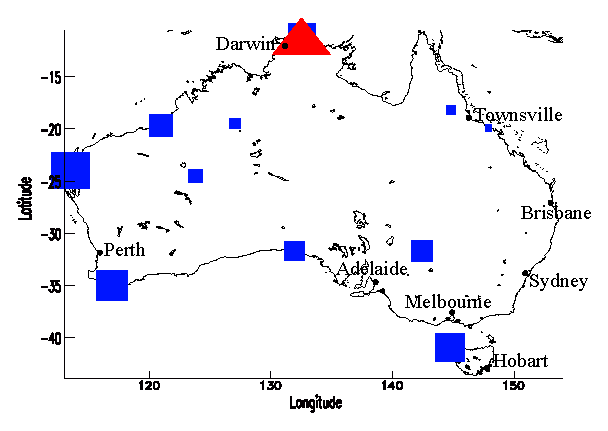
\includegraphics{Figures/asympt_config_full_II_11point_wind_21point_dsr_exclusion_raw_demand}\caption{Map of the optimised installed capacity for the whole-country simulation.
Blue squares represent wind capacity, the red triangle solar capacity,
and the size of the shape indicates the size of the installation relative
to the largest. The largest square is 12GW and the triangle is 23
GW. Some of the major population centres are also labeled for reference.
\label{fig:All-Aus-Installed-Cap}}
\end{figure}
\begin{figure}[H]
\noindent \begin{centering}
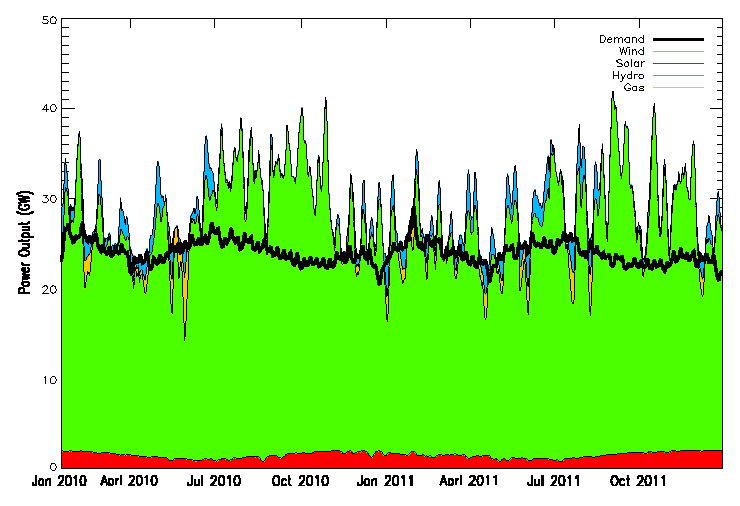
\includegraphics{Figures/GA_output_CoV_proxim_penalty_polyfill_ACCESS_scaled_cost_asympt_config_full_II}
\par\end{centering}

\caption{Time series output of the optimised solution for the whole-country
simulation. Output is daily averaged and the time series of each resource
is plotted on top of the previous. Hydro (blue) below the demand curve
(black) represents water being released downhill while the reverse
(pumping uphill) is true for hydro above the demand curve.\label{fig:All-Aus-Time-Series}}
\end{figure}


What is also evident from Figs. \ref{fig:All-Aus-Installed-Cap} and
\ref{fig:All-Aus-Time-Series} is the use of very remote locations
in Western Australia (WA). It is concluded that these locations in
WA have very complementary resources---and thus minimise the gas usage
in the model (cost effective given the high costs of gas). Interesting
to note, however, is the reliance on only one solar station (near
Darwin). This location is part of a region in north-west Australia
that has the highest annual solar irradiance of all Australian locations
(as seen earlier in Fig. \ref{fig:solar-avg-bom}). There is evidently
no advantage for the electricity model to connect another solar location.
Instead, all of the solar electricity needed is simply installed in
one of the locations with the highest average output (the near-Darwin
location seen in Fig. \ref{fig:All-Aus-Installed-Cap}). 

In general, solar is seemingly under-utilised. There appears to be
no advantage in relying more heavily on solar electricity. This result
is repeated throughout the thesis (see later sections) and is also
concordant with other high renewable electricity dependent studies
of Australia (for instance, \citealp{Elliston2013}). The inability
of the solar resource to provide electricity at night and the lack
of diversity in resource indicates its large-scale use without storage
could be limited in the future. Analysis not presented in the thesis
showed that no realistic level of penalty could be employed to eliminate
the use of remote Western Australian locations. This result, while
less informative for the future design of Australia\textquoteright{}s
RE capacities (due to the vast distances from important load centres),
is potentially very instructive for the resource assessment of Australia.
That is, when given the opportunity to install renewable capacity
across Australia the electricity model chooses to use many remote
Western Australian locations for renewable capacity. Consequently,
any future scenarios that limit the site selection to eastern Australia
will have to rely on less diverse and less effective locations. The
next section explores the implications of this finding by limiting
the electricity model's choice of locations to only those in eastern
Australia (the NEM).


\section{NEM-Only Simulations\label{sec:NEM-Only-Simulations}}

This section examines a simulation of the electricity model utilising
only locations from eastern Australia (the NEM). It is assumed that
limiting available sites to the south and east will produce a more
realistic map of installed capacities for Australia, thus making later
conclusions surrounding moments of low wind and solar and the most
influential synoptic weather regimes, more realistic. 


\subsection{Limiting site selection\label{sub:NEM-Site-Selection}}

Figs. \ref{fig:NEM-Only-RegGrid}a and \ref{fig:NEM-Only-RegGrid}b
show the NEM-only solar and wind sites to be optimised. The sites
were selected based on the state borders of Australia such that only
sites from the original array that were contained within the borders
of South Australia, Victoria, Tasmania, New South Wales and Queensland
were included. Thus the same minimum distance and land availability
restraints introduced earlier are also relevant for the NEM-only simulations.
\begin{figure}[H]
\noindent \begin{centering}
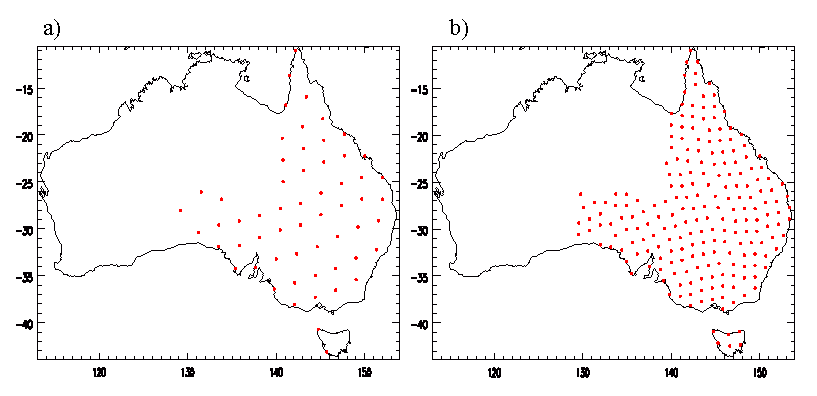
\includegraphics{Figures/RegGrid_locals_dsr_21point_gap_filtered_east-states}
\par\end{centering}

\caption{The sites (red dots) from within the ACCESS-A grid selected for the
NEM-only simulations. a) is the map of solar stations and b) the map
of wind stations. \label{fig:NEM-Only-RegGrid} }
\end{figure}



\subsection{Mapping between ACCESS and ERA-Interim\label{sub:ACCESS-ERA-Mapping}}

An important step for later analysis was the identification of synoptic
regimes as they occurred in 2010-2011. Part 2 identifies the occurrence
of 30 synoptic weather regimes by utilising the results from Part
1---the 30-node SOM that was created from ERA-Interim MSLP data. It
was necessary to assign all ACCESS-A time steps with a SOM node from
Part 1 in order to form relationships between moments of low output
from the ACCESS-optimised network and the large-scale weather regimes
that co-occur. A fundamental component of this thesis is the influence
of synoptic scale variability on RE output. The SOM nodes represent
common synoptic scale conditions and provide the link between synoptic
scale variance and RE output.

In order to utilise the Part 1 SOM, ERA-Interim data for 2010-2011
was obtained. The assigning of SOM nodes to 2010-2011 ERA-Interim
data occurred as per Part 1 whereby the closest matching SOM node
(the Best Matching Unit (BMU)) was assigned to each ERA-Interim time
step in 2010-2011. A filtering process was also undertaken to eliminate
time steps that had ambiguous relationships to the SOM. The level
of filtering used in Part 2 involved the elimination of BMUs that
had a single-point discrepancy of more than 20hPa, a further elimination
of the worst 5\% of remaining BMU and a final checking procedure with
a 4hPa exceedance threshold (refer to Section. \ref{sub:Filtering-the-Mapping}
for a detailed description of these filtering measures). The filtering
process with the 2010-2011 ERA-Interim data eliminated just over 6\%
of matches. 

Following this, the mapping from ERA-Interim temporal resolution,
which is six-hourly, to ACCESS temporal resolution, which is hourly
(and also incomplete), was necessary. The mapping allows for the assignment
of a SOM node from the list of filtered BMU to each available ACCESS-A
time step. The process of matching hourly resolution data to six-hourly
resolution data was undertaken by simply allocating blocks of six
hours from ACCESS-A that were centred on an ERA-Interim time step
(see Fig. \ref{fig:ERA-ACCESS-TS-Map} for a graphical example). Given
that within any block of six ACCESS-A time steps there is only one
hour that matches exactly the hour of the ERA-Interim time step some
unevenness in the six-hour block was inevitable. The decision was
made to implement a \textquoteleft{}forward-leaning\textquoteright{}
approach. The forward leaning approach involved assigning the previous
two hours, the hour that matched the ERA-Interim time step and the
next three hours from ACCESS-space to each ERA-interim time step.
\begin{figure}[H]
\noindent \begin{centering}
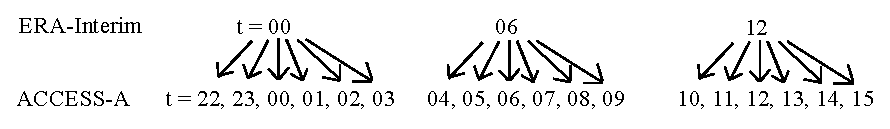
\includegraphics{Figures/Mapping_ts}
\par\end{centering}

\caption{Graphical example of the mapping between ERA-Interim and ACCESS-A.
The units for t are in hours UTC.\label{fig:ERA-ACCESS-TS-Map}}
\end{figure}


The result of this procedure was the formulation of an hourly-resolved
series of ERA-Interim derived SOM node occurrences. In order to show
the remarkably close relationship between wind/solar availability
for each synoptic regime in Part 1, with that of Part 2, Fig. \ref{fig:ACCESS-SOM-Bivar}
illustrates the average capacity of wind/solar from the ACCESS-A data,
but for the synoptic regimes classified with the ERA-Interim data
from Part 1. Comparing Fig. \ref{fig:ACCESS-SOM-Bivar} with the associated
plot from Part 1 (Fig. \ref{fig:SOM-Bivar-Wind-Solar}) illustrates
on the whole concordant wind/solar average capacity in the ACCESS-A
data. That is, in the ACCESS-A data the summer-only nodes have, in
general, regions of high concurrent wind and solar capacities and
the region that encompasses nodes eight, nine, 14, 15 and 21 has very
limited wind and solar availability.
\begin{figure}[H]
\noindent \centering{}\includegraphics{Figures/ACCESS_average_capacity_per_node-wind_solar_RGB_middle}\caption{Average 2010-2011 ACCESS-A wind and solar capacity associated with
the occurrence of SOM nodes from the SOM in Part 1 (Fig. \ref{fig:SOM-Bivar-Wind-Solar}).
Wind capacity is in terms of power and solar capacity is in terms
of the highest DSR value from the 2010-2011 data set. Locations that
have a colour with an increasing blue component represent higher wind
capacities and an increasing red component higher DSR capacities---purple
indicates a location with high average wind and DSR capacity. \label{fig:ACCESS-SOM-Bivar}}
\end{figure}



\subsection{Results Using a Standard Transmission Cost\label{sub:NEM-Only-Standard-Transmission}}

This section presents results from an optimisation of the east-Australian
sites (Fig. \ref{fig:NEM-Only-RegGrid}). Although it was possible
to present many different simulations with similar configurations,
what is presented in this section is a representative simulation using
the two-years of data available from the ACCESS-A model. What was
found in this study, and the study by \citet{Elliston2012}, was a
very small variation from run-to-run using the GA. That is, the final
optimal cost function value found by the GA was relatively insensitive
to variations in starting position of the GA population (the random
initialisation). Using a transmission cost for high-voltage DC cabling
of \$1M/Km (\citealp{Humpert2012}) the optimal placement of renewable
resources is shown in Fig. \ref{fig:NEM-Only-Installed-Cap}.
\begin{figure}[H]
\noindent \centering{}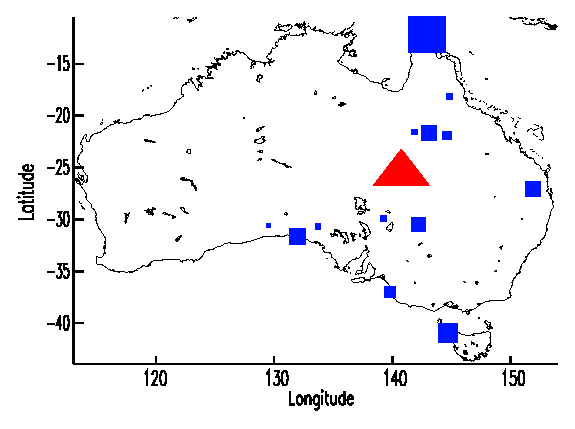
\includegraphics{Figures/asympt_config_full_NEM_east-states_11point_wind_21point_dsr_exclusion_raw_demand}\caption{Installed capacity location and size for the NEM-only simulation.
Coloured shapes are as per Fig. \ref{fig:All-Aus-Installed-Cap} except
the largest square is 17.3GW of wind and the triangle is 5.4GW of
solar. \label{fig:NEM-Only-Installed-Cap}}
\end{figure}
\begin{figure}[H]
\noindent \centering{}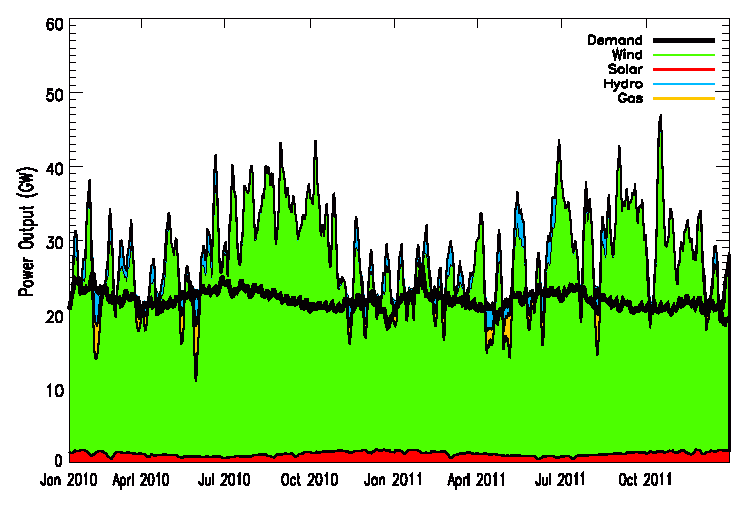
\includegraphics{Figures/GA_output_asympt_config_full_NEM_east-states_dist-penlty}\caption{Daily-averaged time series output from the NEM-only simulation.\label{fig:NEM-Only-Time-Series}}
\end{figure}


The costs and GA configuration used for the simulation presented in
this section are the same as the whole-country simulation (Table.
\ref{tab:Aus-Wide-Config-Parms}), and the installed capacities are
outlined in Table. \ref{tab:NEM-Only-Resource-Stats}.
\begin{table}[H]
\noindent \begin{centering}
\begin{tabular}{|c|c|c|}
\hline 
Resource: & Capacity (GW): & Capacity Factor (\%):\tabularnewline
\hline 
Solar & 5.4 & 20.8\tabularnewline
\hline 
Wind & 76 & 35\tabularnewline
\hline 
Hydro & 5 & 22.3\tabularnewline
\hline 
Gas & 16.7 & 4.1\tabularnewline
\hline 
\end{tabular}
\par\end{centering}

\caption{Resource statistics for the NEM-only simulation. Capacity factor is
the total output as a percentage of the output had the resource been
operating at capacity for all times.\label{tab:NEM-Only-Resource-Stats}}
\end{table}
 

The installed capacities needed by each resource are quite similar
to those outlined in studies of the same region (\citealp{AEMO2013};
\citealp{Elliston2012}). The costs used are also of the same order
as those used in the \citet{AEMO2013} and \citet{Elliston2013} studies---providing
confidence in their realism. Figs. \ref{fig:NEM-Only-RegGrid} and
\ref{fig:NEM-Only-Time-Series} illustrate the installed capacities
and time series output from the optimised solution, respectively.
What is clear from Fig. \ref{fig:NEM-Only-Time-Series} is the increase
in oversupply from the renewables when compared to the earlier simulation
of the whole continent (maximum oversupply increased from 34GW to
49GW). This was not unexpected given the similarity in technology
costs between the two simulations and the greater diversity in resources
available in the whole-country simulation. Table. \ref{tab:NEM-Only-Resource-Stats}
shows there is a similar reliance on wind electricity in the NEM-only
simulation when compared to the study by \citet{Budischak2013} (meeting
demand from north-east USA with RE). What is clear in both this study
and the \citet{Budischak2013} study is that wind electricity is favoured
for its load-matching abilities and solar PV electricity is less favoured
because of its inability to meet demand at night. What is also clear
from Fig. \ref{fig:NEM-Only-Installed-Cap} is the choice of some
remote locations in spite of the extra transmission cost of connecting
these sites. The largest wind site (17.3GW in northern Queensland)
is a long distance from the nearest capital city (Townsville) and
the largest solar installation (5.4GW in south-west Queensland) is
also quite a distance from the nearest capital city (Brisbane). Thus
there still appears to be a tendency by the GA to prefer locations
with decent/complementary resources over those that might be closer
to a capital city, but whose resources are not as optimal. This could
indicate a connection cost that is too inexpensive or alternatively
a resource that is far superior to alternative locations. The answer
to this question is addressed in later sections where the connection
cost is increased (see sections \ref{sub:2X-Optimisation} - \ref{sub:8X-Optimisation}).
The results illustrated in Figs. \ref{fig:NEM-Only-Installed-Cap}
and \ref{fig:NEM-Only-Time-Series} were obtained using a connection
cost that was concordant with values suggested in \citet{Humpert2012}.


\subsection{Identifying Low Renewable Electricity Output Events\label{sub:Low-RE-Definition}}

This section describes the process used to identify events from the
NEM-only solution that were deemed to be of \textquoteleft{}low\textquoteright{}
renewable electricity (low RE) output. The identification of a low
RE event is described in the following process: 
\begin{itemize}
\item Any ACCESS-A time step that had a combined RE output that was more
than 20\% below demand was said to be a low RE time step. 
\item An event was deemed to be a collection of consecutive low RE time
steps. Except where: 

\begin{itemize}
\item The next low RE time step is within six hours of the previous low
RE time step 
\end{itemize}

OR 
\begin{itemize}
\item A time step is within six hours of the nearest low RE time step and
only just failed the original criterion of being more than 20\% below
demand. The definition of only just failing was deemed to be a time
step where the combined RE output was more than 15\% below demand. 
\end{itemize}
\end{itemize}
The 20\% below threshold was relaxed to 15\% in the above in order
to increase the continuity of events. 20\% below demand was seen as
an appropriate figure, but should (for example) a time step only just
fail this criterion and was a critical time step for continuing a
new event or not, it should be included. This process could be seen
as similar to smoothing the time series of low RE by applying a running
mean and then only including smoothed time steps below the original
80\% of demand criterion. The approach presented here is also similar
to that undertaken by \citet{AEMO2013} in their simulation of 100\%
RE for the NEM. \citet{AEMO2013} analysed what they termed to be
the most challenging week of their simulation. The definition of the
most challenging week in \citet{AEMO2013} was that which used the
most gas back-up. AEMO's definition is intuitively similar to that
outline above given that the moments of low RE output would also correlate
well with increased gas usage to cover the gaps in RE---although modulated
depending on the state of the hydro reserves. Once the low RE time
steps and events from the NEM-only simulation were identified the
next step was to analyse their relationship to the large-scale synoptic
weather patterns.


\subsubsection{Analysis of Weather Systems Associated with Low RE Events\label{sub:Low-RE-SOM-Analysis}}

This section describes the association between the occurrence of the
synoptic regimes identified by the SOM from Part 1 and the low RE
time steps and low RE events from the NEM-only simulation. Fig. \ref{fig:Low-RE-SOM-Percentage-Plot}
outlines the percentage of very low RE time steps that co-occur with
the SOM nodes identified in Part 1. Very low RE was deemed to be the
lowest 20\% of low RE time steps. The data used in Fig. \ref{fig:Low-RE-SOM-Percentage-Plot}
encompasses the lowest 20\% of low RE time steps. Plotting of just
the association between low RE and the SOM showed some significant
relationships (not shown), however plotting of the worst 20\% (Fig.
\ref{fig:Low-RE-SOM-Percentage-Plot}) showed more clearly the regions
of the SOM/synoptic types that were problematic, as well as those
regions that were not problematique. Fig. \ref{fig:Low-RE-SOM-Percentage-Plot}
indicates that there were a few SOM nodes that were either significantly
associated (significantly high percentage) or significantly unassociated
(significantly low percentage) with low RE time steps.
\begin{figure}[H]
\noindent \centering{}\includegraphics{Figures/asympt_config_full_NEM_east-states_events_20perc_below_demand_som_occurrence_perc_ERA-Int_6x5_alpha0\lyxdot 5_bubble_cont}\caption{Percentage occurrence of very low RE time steps that are associated
with each SOM node from Part 1. Only time steps from the lowest 20\%
of low RE time steps were used (worst of the worst). Red colours represent
significantly high associations and blue colours significantly low
associations. Significance is measured at the 5\% level using a two-tailed
Monte-Carlo simulation and darker grey indicates larger values.\label{fig:Low-RE-SOM-Percentage-Plot}}
\end{figure}


Significance testing was undertaken via the bootstrapping/Monte-Carlo
approach (Chapter 5.3.3 from \citet{Wilks2011}). The occurrence of
SOM nodes in time was randomised in order to assess the chance that
such relationships between low RE and SOM node were possible, at some
significance level, by random. The randomising was also weighted by
the transition matrix for the 2010-2011 period (see ahead, Fig. \ref{fig:All-ERA-SOM-Transitions}),
which ensures that physically realistic time series were created---or
rather, time series where the autocorrelation in the MSLP field is
taken into account. As a consequence of the bootstrapping process
a new time series of SOM node occurrences was formed. The new time
series was then filtered such that the same moments in time eliminated
in the original filtering process were also eliminated in the randomised,
or altered, version. 10,000 altered versions were then created and
for each node (1-30) it was possible to create a distribution (one
member for each altered version) of the percentage occurrence with
low RE time steps (Fig. \ref{fig:Low-RE-SOM-Percentage-Plot}). If
the measured percentage occurrence was in either tail of the distribution
(2.5\% of the distribution in each tail) the actual occurrence was
said to be significant at the 5\% level. 

In particular, there were some SOM nodes that appeared to never co-occur
with very low RE for the NEM-only simulation. Nodes six and 25 significantly
never co-occured with the lowest RE output. However, of more interest
were perhaps those nodes that were significantly associated with very
low RE output. For instance, there was a region of the SOM (nodes
eight, nine, 10, 15) that represents almost half of all of the very
low RE time steps. Given the smooth nature of the SOM these nodes
represent similar MSLP distributions and therefore represent a sub-set
of similar synoptic regimes from within the SOM that were associated
with over one third of all very low RE time steps. Another important
association seen in Fig. \ref{fig:Low-RE-SOM-Percentage-Plot} was
that of node 30, which at 8.5\% of the lowest RE time steps also represented
a notable cluster, despite not passing the 5\% test. Node 30, as was
seen in Part 1, is a summer-time node and is also quite far removed
from the significant sub-set of nodes (eight, nine, 10 and 15). In
the next section further analysis of two nodes and their association
with very low RE for the NEM-only simulation is presented---nodes
nine and 30, as these represent the two most notable regions of the
SOM. 


\subsubsection{Node nine analysis\label{sub:Node9-Low-RE}}

The next two sections analyse nodes nine and 30 and their relationship
to very low renewable electricity output. In particular, any meteorological
reasons for why these synoptic regimes are problematic for the optimised
NEM-only simulation.
\begin{figure}[H]
\noindent \begin{centering}
\includegraphics{Figures/mslp_average_sig-hatching_node_9_asympt_config_full_NEM_east-states_for_lowest_20perc_of_renew_events_20perc_below_demand}
\par\end{centering}

\caption{MSLP composite of node nine events that co-occur with very low RE
output. Stippling indicates features that are statistically significantly
different from the long-term (ERA-Interim 1989-2009) average of MSLP
using a two-tailed test at 0.05.\label{fig:Node9-Low-RE-MSLP-Composite}}
\end{figure}


Above is the MSLP composite for SOM node nine when it is said to co-occur
with very low RE output (Fig. \ref{fig:Node9-Low-RE-MSLP-Composite}).
Similar to the map of node nine from the SOM of Part 1 (Fig. \ref{fig:6x5-SOM-space-Cont})
the composite of very low RE for node nine is characterised by a relatively
weak centre of high pressure just off the coast of Western Australia
and occurs predominantly in late Austral Autumn (May-June). Stippling
in Fig. \ref{fig:Node9-Low-RE-MSLP-Composite} shows areas that have
an MSLP value significantly different from the long-term mean MSLP
for that location. The long-term mean was taken as the average value
from the available ERA-Interim data-set of Part 1 (1989-2009). The
significance test was a comparison of means as outlined in \citet{Wilks2011}
(one mean from the 1989-2009 period and the other from the very low
RE grouping of node nine).
\begin{figure}[H]
\noindent \centering{}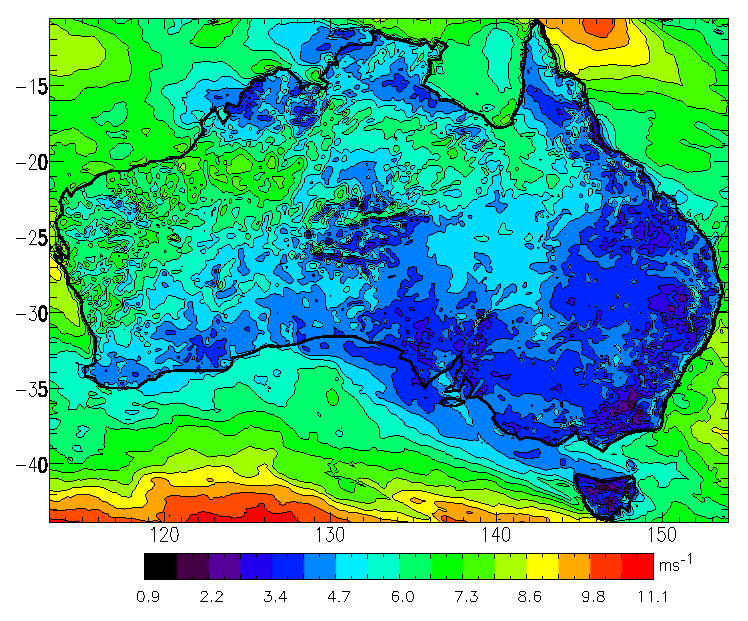
\includegraphics{Figures/u80_node_9_asympt_config_full_NEM_east-states_for_lowest_20perc_of_renew_events_20perc_below_demand}\caption{Composite 80m wind speed for the occurrences of node nine that co-occur
with very low RE output in the NEM-only simulation.\label{fig:Node9-LowRE-U80-Composite}}
\end{figure}
 

In fact, the map of node nine in Fig. \ref{fig:Node9-Low-RE-MSLP-Composite}
shows relatively weak pressure gradients over most of the Australian
domain---most of which are significant features. The weak pressure
gradients could be an artifact of the averaging process undertaken
when producing the composite. However, short of showing each member
of the composite or a figure of the standard deviation at each point,
the associated average 80m wind speed is shown in Fig. \ref{fig:Node9-LowRE-U80-Composite}---it
was expected that given the relationship between large-scale pressure
and the geostrophic wind there might also be weak wind speeds associated
with the very low RE occurrences of node nine. As is seen in Fig.
\ref{fig:Node9-LowRE-U80-Composite} there are indeed very weak average
wind speeds across most of the eastern part of Australia during very
low RE node nine. The availability of wind speeds above the cut-in
of 3m/s is remarkably low. In an average sense it would actually be
expected that an occurrence of very low RE node nine might produce
almost no power across eastern Australia. This is significant given
the positioning of resources for the NEM-only simulation. It appears
as if the low pressure gradients associated with node nine, and in
particular very low RE node nine, are quite detrimental for the optimised
resources from the NEM-only simulation. The emphasis here being that
the resources allocated by the electricity model are optimised. Thus
there appears to be no net advantage in the model avoiding this type
of stilling weather pattern---the very low RE node nine is likely
not a significant enough portion of the hours in 2010-2011 to warrant
changing the resource allocation to accommodate it. 
\begin{figure}[H]
\noindent \centering{}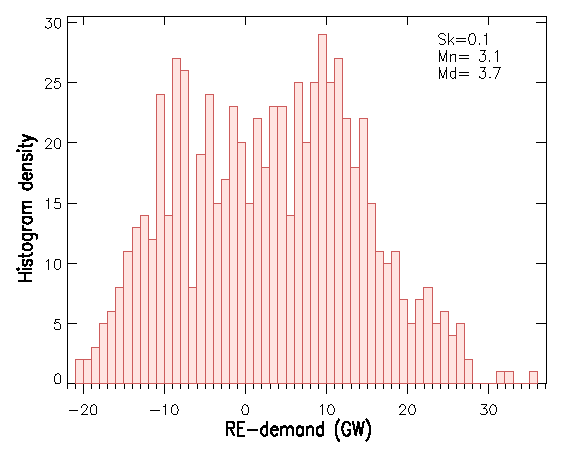
\includegraphics{Figures/Node_9_histogram_demand-RE}\caption{Distribution of RE - demand when node nine occurs in the NEM-only
simulation. Histogram density indicates the number of hours in the
NEM-only simulation where node nine is either over or under producing
with RE in comparison to demand. Distribution characteristics appear
top-right where Sk is Skewness, Mn is Mean and Md is Median.\label{fig:Node9-RE-Demand-Histogram} }
\end{figure}


To investigate the characteristics of node nine and its influence
on all hours in the two-year simulation Fig. \ref{fig:Node9-RE-Demand-Histogram}
illustrates the distribution of RE - demand when node nine is said
to occur. As can be seen from Fig. \ref{fig:Node9-RE-Demand-Histogram}
there is actually no real bias suggesting node nine is particularly
detrimental, even on average. Fig. \ref{fig:Node9-RE-Demand-Histogram}
shows the skewness of RE - demand for node nine is almost zero and
the mean and median are also in close association. In this instance
the predictive power of node nine is limited. The spread of possible
values seen in Fig. \ref{fig:Node9-RE-Demand-Histogram} suggests
that the variance around node nine is large and both extremes (oversupply
and undersupply) are possible. The importance of node nine is the
occurrence of the very low output potential, which is identified by
the version of node nine seen in Fig. \ref{fig:Node9-Low-RE-MSLP-Composite}
with very low pressure gradients. Thus the conclusions for node nine
are:
\begin{itemize}
\item The association with very low RE is significant
\item Node nine has the potential to be detrimental to wind power for nearly
the entire NEM region
\item However node nine is not always associated with very low RE---node
nine is also associated with oversupply. Oversupply of RE also involves
the relative production of solar and wind. For instance, solar is
less directly influenced by MSLP gradients, indicating that weak pressure
gradients from node nine could also lead to RE oversupply.
\end{itemize}

\subsubsection{Node 30 analysis\label{sub:Node30-Low-RE}}

Node 30 was also seen as being notably associated with very low RE
output from the NEM-only simulation (8.5\% of very low RE hours).
However, node 30 is from a different region of the SOM and represents
a different synoptic regime to node nine. Node 30 is characterised
by lower pressure over WA (Fig. \ref{fig:Node30-Low-RE-MSLP-Composite})
and occurs predominantly in late Austral Summer (Feb-March). 
\begin{figure}[H]
\noindent \centering{}\includegraphics{Figures/mslp_average_sig-hatching_node_30_asympt_config_full_NEM_east-states_for_lowest_20perc_of_renew_events_20perc_below_demand}\caption{As per Fig. \ref{fig:Node9-Low-RE-MSLP-Composite}, except for the
occurrences of node 30 that co-occur with very low RE.\label{fig:Node30-Low-RE-MSLP-Composite}}
\end{figure}


Nearly all of the domain for the composite of very low RE node 30
is significantly different to the long-term MSLP. Node 30 could be
considered as a continental heat low, which also occur in summertime
(\citealp{Sturman2005}). Continental heat lows form as a result of
convection that is triggered by heating of the continent---hence the
association with summer. The low pressure centred over WA represents
a break between successive high pressure systems, which are visible
in the eastern and western edges of the domain (Fig. \ref{fig:Node30-Low-RE-MSLP-Composite}).
Node 30, as per node nine, is also characterised by low pressure gradients
across the Austral domain. In fact, the pressure gradients for very
low RE node 30 are actually weaker than that seen for very low RE
node nine. Again, this results in, on average, large-scale stilling
over the NEM region (Fig. \ref{fig:Node30-LowRE-U80-Composite}).
The weak 80m wind speeds seen for very low RE node 30 appear to be
quite similar to node nine---in spite of any difference in weather
type and MSLP distribution. For very low RE node 30 there is limited
access to average wind speeds above about 5 ms\textsuperscript{-1}
for most of the Australian continent and limited access to wind speeds
above the turbine cut-in 3 ms\textsuperscript{-1} for the NEM. Fig.
\ref{fig:NEM-Only-Installed-Cap}, which shows the allocation of resources
for the NEM-only simulation, had the largest installation of wind
speed in northern Queensland. This region, for both very low RE node
nine and node 30, is particularly subject to average wind speeds less
than the cut-in. It is concluded that this is why these occurrences
of nodes nine and 30 are identified as very low RE. However, an important
point to make is that Figs. \ref{fig:Node30-LowRE-U80-Composite}
and \ref{fig:Node9-LowRE-U80-Composite} show no realistic alternative
(in terms of a location that could avoid the stilling). One might
also argue that these significant node-low RE associations are of
no concern because the NEM-only simulation is not realistic/comprehensive
enough and would therefore never be implemented. What this argument
misses, however, is the fact that the low wind speeds seen in Figs.
\ref{fig:Node30-LowRE-U80-Composite} and \ref{fig:Node9-LowRE-U80-Composite}
would be detrimental for almost any arrangement of resources across
the NEM. Thus, if a somewhat simplistic, or \textquoteleft{}best-case
scenario\textquoteright{} simulation---like that of the NEM-only simulation---fails
to accommodate these stilling synoptic regimes than surely a more
sophisticated simulation (that would also be more limited in its choices
for resource allocation) would also perform poorly under these conditions,
as well as others.
\begin{figure}[H]
\noindent \centering{}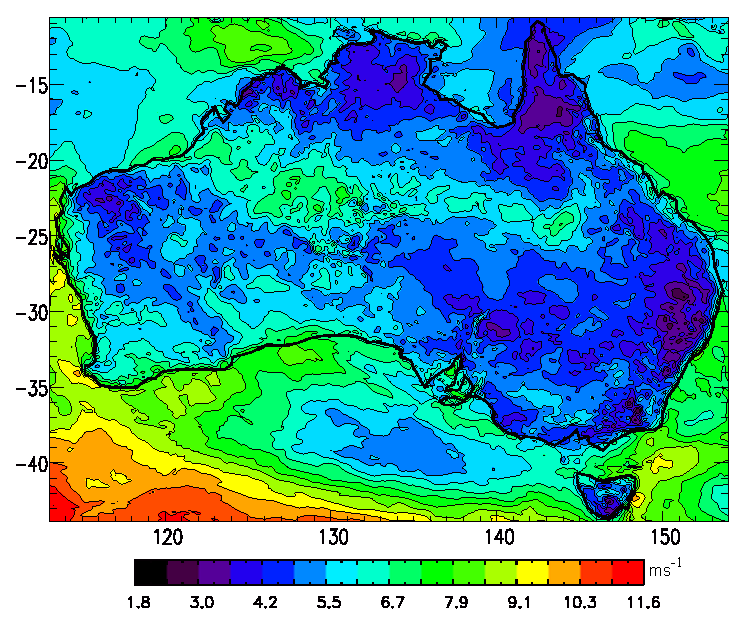
\includegraphics{Figures/u80_node_30_asympt_config_full_NEM_east-states_for_lowest_20perc_of_renew_events_20perc_below_demand}\caption{As per Fig. \ref{fig:Node9-LowRE-U80-Composite}, except for Node
30.\label{fig:Node30-LowRE-U80-Composite}}
\end{figure}
\begin{figure}[H]
\noindent \begin{centering}
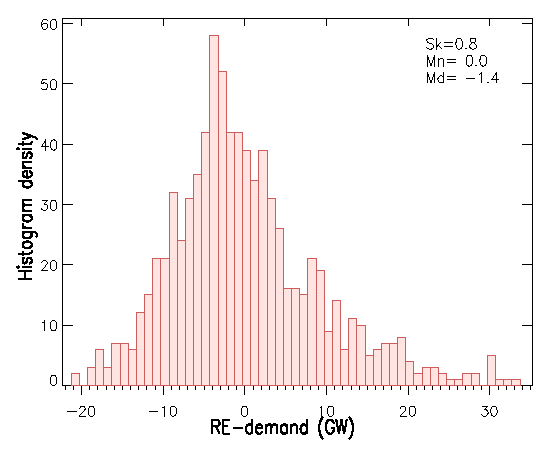
\includegraphics{Figures/Node_30_histogram_demand-RE}
\par\end{centering}

\caption{As per Fig. \ref{fig:Node9-RE-Demand-Histogram}, except for the distribution
for node 30.\label{fig:Node30-RE-Demand-Histogram}}
\end{figure}
 

The distribution of RE - demand for all occurrences of node 30 shows
more of a significant bias towards very low RE than node nine with
a median of -1.4GW and a mean of 0GW, but again no conclusion that
node 30 is significantly more associated, on the whole, with very
low RE than high (Fig. \ref{fig:Node30-RE-Demand-Histogram}). However,
when analysing similar distributions for all nodes it becomes clear
that there are some nodes (seen as significantly un-associated with
very low RE in Fig. \ref{fig:Low-RE-SOM-Percentage-Plot}) that have
a bias on the whole towards very high RE output (Fig. \ref{fig:All-Nodes-RE-Demand-Hist}).
For instance, nodes six and 25 were seen as never occurring with very
low RE for the NEM-only simulation. These nodes also have a mean over-supply
(when considering all occurrences from the two years) of about 14.5GW
and very limited occurrences of under-supply. Other nodes that were
also significantly un-associated, but in a non-zero sense, with very
low RE output have very high means in terms of oversupply (Fig. \ref{fig:All-Nodes-RE-Demand-Hist}).
These nodes include node 19 (mean of 13.9GW) and node four (mean of
9.5GW). While oversupply is more manageable for an RE-based electricity
network than undersupply, the extent to which nodes six and 25 are
associated with oversupply is remarkable; these nodes are analysed
in section \ref{sub:High-RE-Nodes6-25}.
\begin{figure}[H]
\noindent \centering{}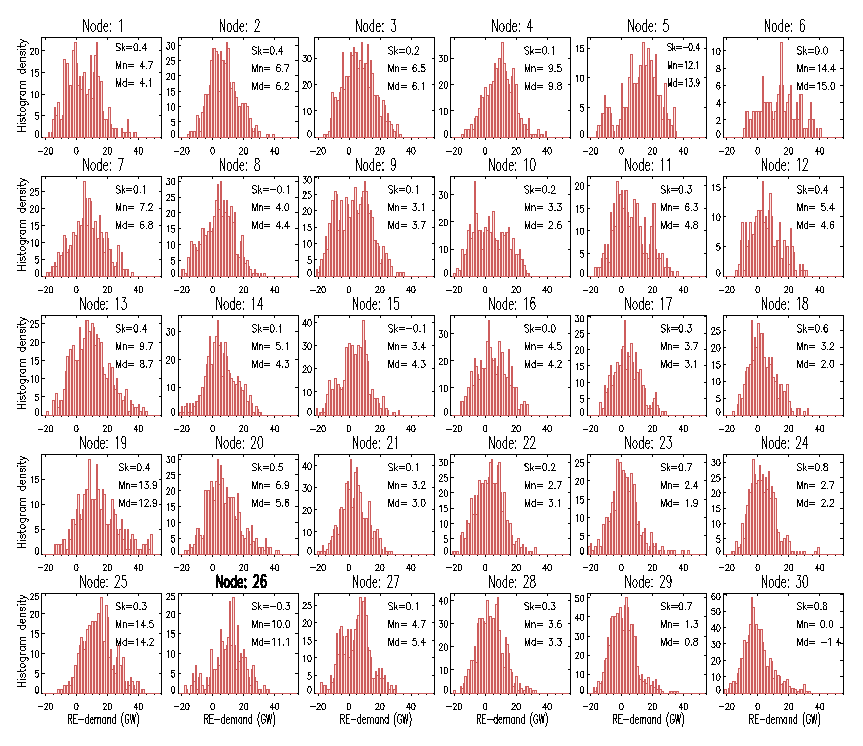
\includegraphics{Figures/All_nodes_histogram_demand-RE}\caption{Histogram of RE - demand for all nodes during the NEM-only simulation.
Sk stands for Skewness, Mn Mean and Md median for each distribution.\label{fig:All-Nodes-RE-Demand-Hist}}
\end{figure}



\subsubsection{Time Series Analysis of the Very Low RE Events\label{sub:Low-RE-TimeSeries-Analysis}}

In terms of the affect on the electrical system, an important consideration
regarding the very low renewable electricity events outlined above
are the return period and duration statistics. In this section analysis
of the temporal characteristics of the very low RE events is presented---extended
periods of very low RE output (see section \ref{sub:Low-RE-Definition}
for the definition of a low RE event). An important consideration
for a future highly RE dependent Australia would be the time wise
behaviour of very low RE output. Characteristics that include average
duration and average return period are important for stability in
output and the potential of black-outs in supply. For instance, \citet{AEMO2013}
in their study of 100\% RE in the NEM noted that managing consecutive
days of low wind and solar output was much more challenging than managing
isolated days of low RE output. What the very low RE event investigation
also provides is the opportunity to analyse whether or not specific
weather regimes re-occur or persist during very low RE events.
\begin{figure}[H]
\noindent \centering{}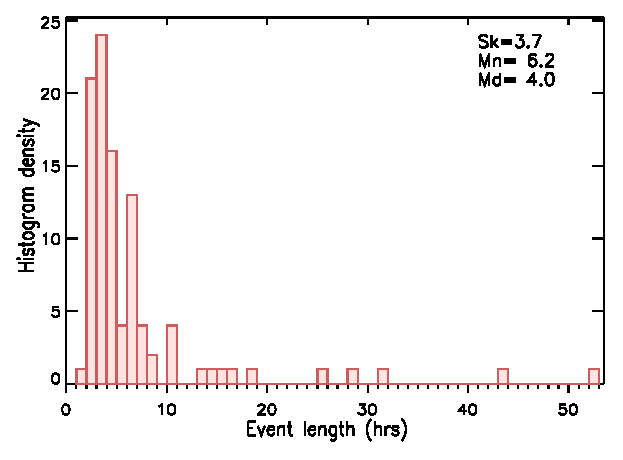
\includegraphics{Figures/Low_RE_events_event_length_histogram}\caption{Distribution of very low RE event lengths for the NEM-only simulation.\label{fig:Low-RE-Event-Length-Histogram}}
\end{figure}
 

Fig. \ref{fig:Low-RE-Event-Length-Histogram} shows the average event
length for the very low RE events in the NEM-only simulation. Fig.
\ref{fig:Low-RE-Event-Length-Histogram} illustrates that there is
a large positive skewness in the event duration as well as a separation
between mean and median. The distribution of event lengths suggests
that events longer than about 10 hours are quite rare---the median
is four hours. However, given the reliability standards of today\textquoteright{}s
NEM (99.998\% of hours met) any event longer than 10 hours would likely
pose significant issues---particularly at peak times. It is clear
that the distribution is skewed by some extreme events that last for,
in the worst case, 52 hours. This is not to suggest that there was
no power available to the NEM for in excess of two days---the definition
of an event is a collection of days where the RE output is more than
20\% below demand---but it does suggest that there is limited supply
in some instances for prolonged periods. In fact, the hydro reserves
would likely run out during a 52 hour event and the system would then
have to rely on expensive gas back-up to meet demand (during the 52
hour event gas peaks at 12.7GW and operates at a capacity factor of
22\%). 
\begin{figure}[H]
\noindent \centering{}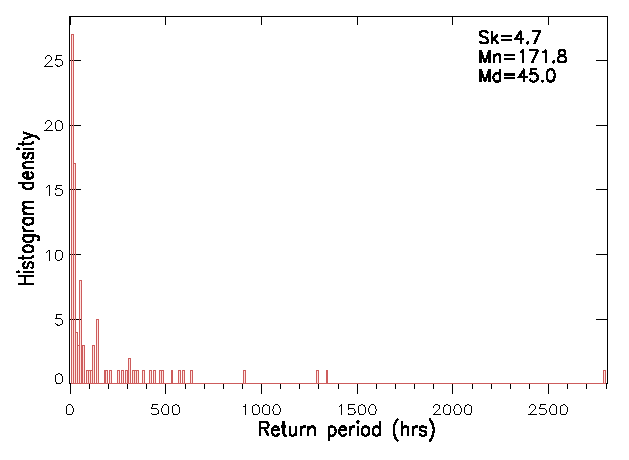
\includegraphics{Figures/Low_RE_events_return_period_histogram}\caption{Distribution of very low RE event return periods for the NEM-only
simulation. A return period is the length of time separating two consecutive
very low RE events. The histogram density shows the number of times
a return period occurs in the NEM-only simulation. \label{fig:Low-RE-Event-Return-Period-Histogram}}
\end{figure}


Fig. \ref{fig:Low-RE-Event-Return-Period-Histogram} illustrates the
average return period for very low RE events in the NEM-only simulation.
The distribution of return period lengths is more skewed than the
event duration distribution and in particular has a very large separation
of the mean and median; indicating that the return period distribution
is even more heavily influenced by extrema. In the case of a return
period distribution, however, a large return period would be considered
positive for the electricity system. In particular the ability of
the electricity system to manage the next moment of low RE output
is aided by a longer return period with increased pumped hydro reservoir
levels. The median return period for a very low RE event is close
to two days at 45 hours (due to the relatively more common return
periods of about two days or less) while the average is closer to
seven days (171.8 hours). The analysis of return periods suggests
that the NEM-only system does in fact have periods during the two
years that have relatively high reliability from RE. That is, there
are some events that are separated by in excess of 20 days and even
one instance where the system went over 116 days without having extended
very low RE. While oversupply might be inevitable for an RE-based
electricity system, oversupply will always be less of an issue than
under-supply. Oversupply is an issue that can be dealt with by a range
of solutions---including curtailment, load shifting and electric car
charging, or other types of storage (like that explored in \citealp{Budischak2013}).
Under-supply, however, has no such easy solution because it is not
possible to simply ramp-up a wind turbine or solar installation when
the wind is low or the sun is not shining. 
\begin{figure}[H]
\noindent \centering{}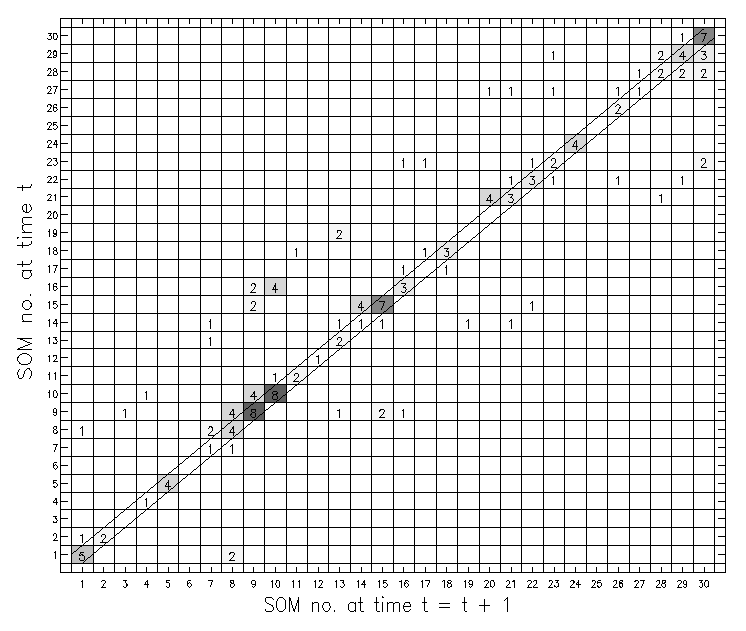
\includegraphics{Figures/asympt_config_full_NEM_east-states_low_re_events_som_transitions}\caption{SOM transition plot for all very low RE events. Numbers show the counts
for each transition within a very low RE event. The original node
number is represented by the vertical axis and the node that is transitioned
to is represented by the numbers in the horizontal axis. No transition
(stationary) is indicated by a coordinate in the diagonal from (1,
1) to (30, 30) and the diagonal is highlighted by the solid transecting
lines.\label{fig:Low-RE-SOM-Transition-Plot} }
\end{figure}


Fig. \ref{fig:Low-RE-SOM-Transition-Plot} shows the persistence or
transitioning of SOM nodes from within the very low RE events of the
NEM-only simulation. Persistence is considered to be an important
characteristic for the identification of synoptic regimes that are
linked to very low RE output. The persistence of a weather type within
a very low RE event could indicate a bias. Such biases are not indentifiable
using statistics, including the Fig. \ref{fig:Low-RE-SOM-Percentage-Plot}
average plots, which aggregate across all low RE events. The definition
of a transition requires that the transition (persistence) be made
within the same very low RE event and that the transition (persistence)
occur to a new (the same) SOM node in six-hourly ERA-Interim space.
For instance, the persistence on a node is not considered to occur
in ACCESS-A space if there is no transition made from hour to hour---a
transition, or not, can only occur across the six-hourly blocks, and,
can only be to a SOM node occurrence that was not filtered out. As
can be seen from Fig. \ref{fig:Low-RE-SOM-Transition-Plot} there
is a lot of persistence or transitions that occur to neighbouring
nodes from within the very low RE events. The banding in Fig. \ref{fig:Low-RE-SOM-Transition-Plot}
that is approximately six nodes apart indicates a transition down/up
the SOM space, rather than across, and is due to the smooth nature
of the SOM. Neighbouring SOM nodes are, by definition, closely related
to each other and thus a transition to a neighbour is by design more
likely. What is also seen in Fig. \ref{fig:Low-RE-SOM-Transition-Plot}
is that nodes nine (high centred south of WA) and 30 (heat low north
west WA) are some of the most persistent. These nodes were seen as
being significantly/notably associated with very low RE output and
Fig. \ref{fig:Low-RE-SOM-Transition-Plot} suggests this is at least
partially due to the persistence of these nodes during an event.
\begin{figure}[H]
\noindent \centering{}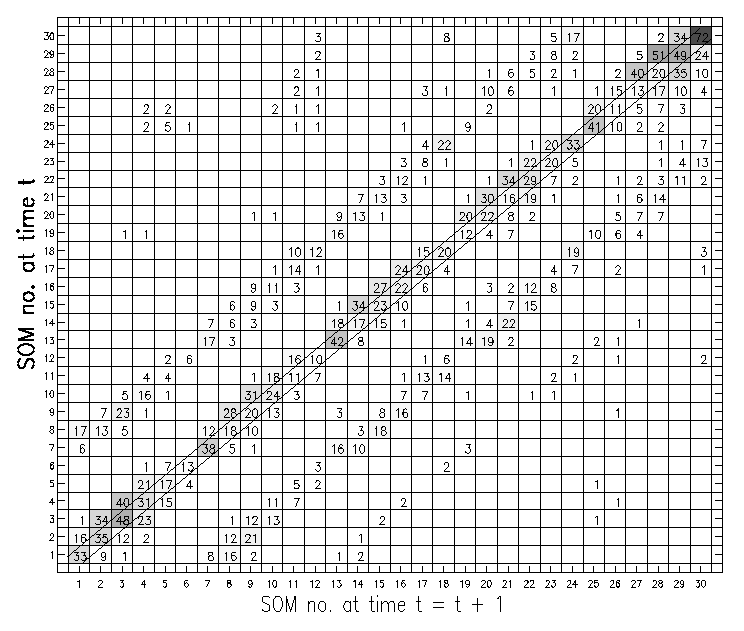
\includegraphics{Figures/asympt_config_full_NEM_east-states_som_transitions_all-ACCESS}\caption{SOM node transitions for all ERA-Interim time steps in 2010-2011.
Solid transecting lines indicate the t=t+1 diagonal.\label{fig:All-ERA-SOM-Transitions}}
\end{figure}


Fig. \ref{fig:All-ERA-SOM-Transitions} shows the persistence during
the whole two year period. Fig. \ref{fig:All-ERA-SOM-Transitions}
clearly illustrates that node 30 is by far the most persistent node
of any of the SOM nodes. This indicates that node 30 is in general
a slow moving synoptic regime---giving an explanation for its persistence
during very low RE events as well. Node nine is, however, the most
persistent node during very low RE events. Yet the persistence of
node nine in general is not as marked as node 30. Thus the southerly
high pressure centre outline in Fig. \ref{fig:Node9-Low-RE-MSLP-Composite}
for node nine has a tendency, at times, of being more persistent.
This observation can help explain the region of significance seen
in Fig. \ref{fig:Low-RE-SOM-Percentage-Plot}. Fig. \ref{fig:Low-RE-SOM-Percentage-Plot}
illustrated that there was a sub-grouping from within the SOM whose
pressure systems were quite similar and who were associated with a
large portion of all very low RE output. Fig. \ref{fig:All-ERA-SOM-Transitions}
suggests this region (nodes eight, nine, 10, and 15) is not particularly
persistent on the whole, but that its persistence is among the highest
during very low RE events (Fig. \ref{fig:Low-RE-SOM-Transition-Plot}).
Thus the southerly high seen for node nine can not only persist for
longer than average but also transition to neighbouring nodes during
a very low RE event.


\subsubsection{Nodes six and 25\label{sub:High-RE-Nodes6-25}}

As can be seen from Fig. \ref{fig:Nodes25_6_RE-Demand-Histogram}a
there is a significant tendency for node 25 to be associated with
oversupply. Earlier analysis of just the very low RE time steps showed
that node 25 never occurred at a time of very low RE. This is easy
to understand when Fig. \ref{fig:Nodes25_6_RE-Demand-Histogram}a
is taken into account. Node 25 has on average 14GW of oversupply when
it occurs, while moments where demand is higher than RE for node 25
are very limited. Fig. \ref{fig:Nodes25_6_RE-Demand-Histogram}b shows
a very similar story of oversupply for node six. On average node six
is associated with 14.4GW of oversupply, and although node six is
less common than node 25, it still shows a very clear bias towards
oversupply. Only 16 time steps are moments of RE below demand for
node six. 
\begin{figure}[H]
\noindent \centering{}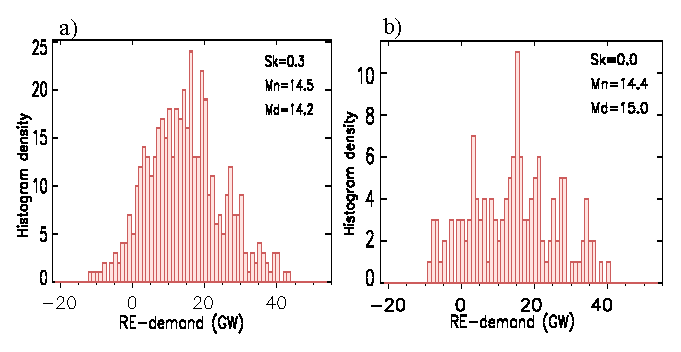
\includegraphics{Figures/Nodes_25_6_histogram_demand-RE}\caption{As per Fig. \ref{fig:Node9-RE-Demand-Histogram},except for a) node
25 and b) node six.\label{fig:Nodes25_6_RE-Demand-Histogram}}
\end{figure}


The synoptic situation for both node 25 and six appears to be quite
similar. Figs. \ref{fig:Node25-MSLP-Composite} and \ref{fig:Node6-MSLP-Composite}
show that node 25 and six are associated with low pressure intrusions
that extend into the southern parts of Australia. Fig. \ref{fig:Node6-MSLP-Composite}
suggests that node six is a more advanced version of node 25 such
that it seems likely node six would follow from node 25 in a normal
westerly progression of synoptic scale systems in the mid latitudes
(although this is not seen in Fig. \ref{fig:All-ERA-SOM-Transitions}).
Node six is associated with low pressure centred south of Adelaide
and an associated front directing cold air to parts of South Australia
and Victoria. Relatively higher pressure gradients also indicate that
node six would be associated with increased wind speeds along the
coast of South Australia, much of Victoria and coastal regions of
NSW. 
\begin{figure}[H]
\noindent \centering{}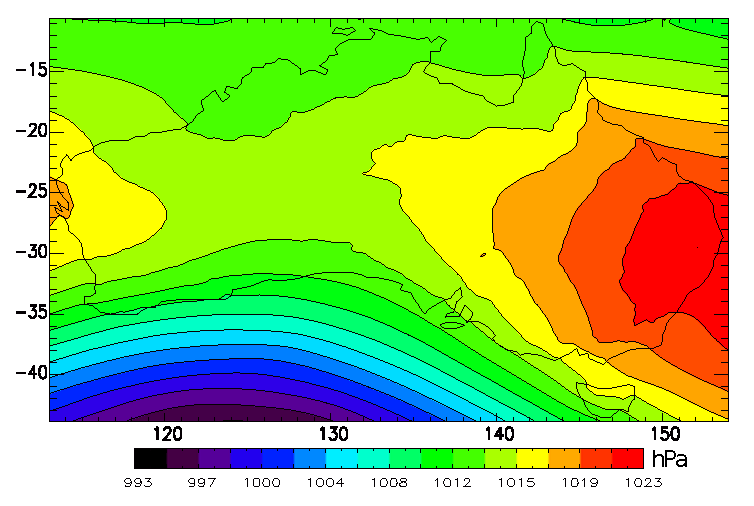
\includegraphics{Figures/mslp_composite_node25}\caption{MSLP composite for all occurrences of node 25.\label{fig:Node25-MSLP-Composite}}
\end{figure}


While node 25 is less associated with low pressure and cold air it
is associated with higher pressure gradients through much of the same
regions as node six. The higher wind speeds are important given the
reliance on wind power in the NEM-only simulation. In particular,
the regions with installed capacity of wind would benefit greatly
from the occurrence of nodes 25 and six. This benefit is apparent
not only in the MSLP plots, but also the oversupply plots shown earlier.
\begin{figure}[H]
\noindent \centering{}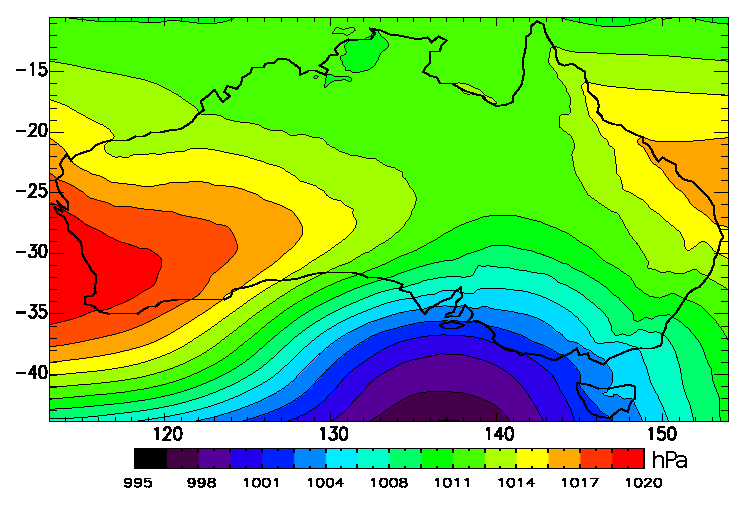
\includegraphics{Figures/mslp_composite_node6}\caption{MSLP composite for all occurrences of node six.\label{fig:Node6-MSLP-Composite}}
\end{figure}


Thus, analysis of SOM node behaviour in combination with the output
of the NEM-Only simulation has been shown to identify common synoptic
regimes that are associated with either favourable or detrimental
RE conditions. Analysis presented in this section indicates that node
nine was significantly associated with, and 30 notably associated
with, very low RE and have the potential to produce large areas of
very low wind speeds across the NEM region. A prediction of nodes
nine or 30, however does not guarantee very low RE as 13\% of node
nine and 8\% of node 30 occurrences were associated with very low
RE. Alternatively, it was shown that a prediction of nodes 25 and
six is far more likely than not to produce conditions that result
in oversupply of wind power in the NEM region. 


\section{Seasonal Optimisations\label{sec:NEM-Only-Seasonal-Optims}}

In this section the influence of the different seasons is identified
by conducting new optimisations of the NEM region, using data only
from one particular season. The following analyses include the Austral
summer (December, January and February) and winter (June, July and
August). It is assumed that optimising just the data for one particular
season will reveal the particular large-scale features that prevail
in that season. For instance, questions (including, is the increase
availability of solar insolation in summer sufficient to overcome
stilling synoptic conditions) regarding the performance of the NEM-Only
simulation that are season-specific can be addressed.

In both the summer-only and winter-only simulations the optimisation
is conducted in the same manner as the NEM-Only simulation (same costs,
cost function formulation, available resource types, etc.) but with
only the data from the 2010-2011 period that fall into that particular
season. Splicing of the data from year to year is conducted such that,
in the case of winter-only, the end of August of 2010 is followed
by the start of June in 2011. Gas costing is also altered slightly
in the season specific simulations. The gas cost structure introduced
in the NEM-Only simulation had a penalty applied to the fuel costs,
which are small for a two-year simulation but would be much larger
over the lifetime of the gas plant. This penalty is increased for
the winter and summer only simulations because they are shorter than
the two-year NEM-only simulation. 


\subsection{Optimisation of the Winter months of 2010-2011\label{sub:Winter-Only-Optim}}

Figs. \ref{fig:Winter-Only-Installed-Cap} and \ref{fig:Winter-Only-Time-Series}
show the installed capacity and time series output for the NEM region
optimisation using the winter ACCESS-A data of 2010-2011. It is immediately
obvious from Figs. \ref{fig:Winter-Only-Installed-Cap} and \ref{fig:Winter-Only-Time-Series}
that the vast majority of installed capacity is located in northern
Queensland and only wind is utilised for the winter-only simulation.
Table. \ref{tab:WInter-Only-Simulation-Stats} shows that there is
an overall reduction in installed capacity of RE (just wind in this
case) for the wintertime optimisation. Table. \ref{tab:WInter-Only-Simulation-Stats}
also suggests that the reliability of the wind resources is higher
in the wintertime---the capacity factor of the total wind speed time
series was 41.2\%, 6\% higher than the NEM-Only simulation.
\begin{figure}[H]
\noindent \centering{}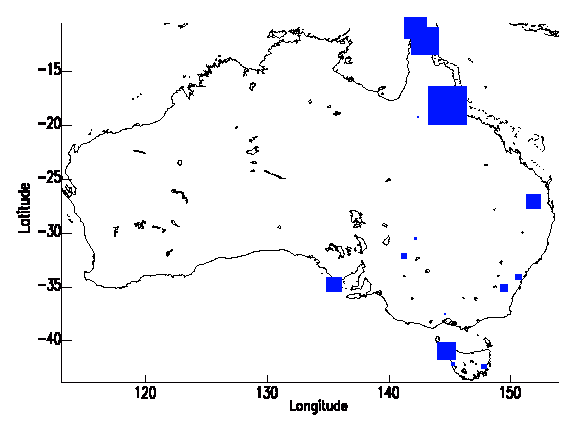
\includegraphics{Figures/asympt_config_full_NEM_east-states_winter-only_11point_wind_21point_dsr_exclusion_raw_demand}\caption{Installed capacity for the winter-only optimisation of the NEM. Blue
squares represent location and size of wind installations, where the
largest square represents 13GW.\label{fig:Winter-Only-Installed-Cap}}
\end{figure}
\begin{figure}[H]
\noindent \centering{}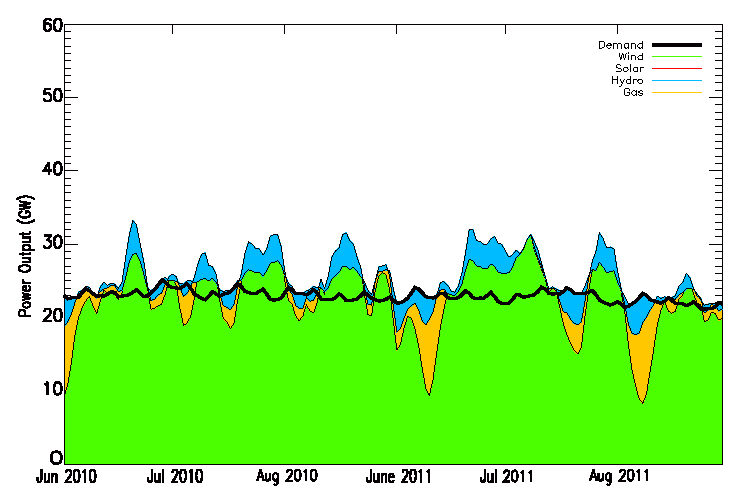
\includegraphics{Figures/GA_output_asympt_config_full_NEM_east-states_winter-only_dist-penlty}\caption{Daily-average time series output for the winter-only optimisation
of the NEM. Hydro (blue) above the demand curve (black) is pumping
uphill while hydro below the demand curve is releasing downhill. \label{fig:Winter-Only-Time-Series}}
\end{figure}


Solar PV is not utilised in the winter-only simulation. The optimisation
process found no advantage in installing solar when given only the
winter conditions, which on average will be lower in terms of surface
insolation due to the positioning of the Sun. The reliability on the
whole is much higher for the winter-only simulation. Despite the winter-only
scenario relying solely on wind power, moments of oversupply for winter-only
peak at less than half that of the NEM-only simulation using all two
years (Table. \ref{tab:Oversupp-Comp-Base-Winter}). Gas, however,
is utilised more in the winter-only simulation---peaking at 18GW and
running at 10\% capacity factor. Thus the winter-only simulation is
able to exploit a more reliable wind resource, but in doing so is
exposed to moments of low output that cannot be covered by excess
hydro reserves and require large amounts of gas back-up. Given that
the results shown in Figs. \ref{fig:Winter-Only-Installed-Cap} and
\ref{fig:Winter-Only-Time-Series} are optimised it can also be concluded
that the cost of installing solar to avoid some of those costly gas
peaks is higher than simply paying for the use of the gas.
\begin{table}[H]
\noindent \begin{centering}
\begin{tabular}{|c|c|c|}
\hline 
Resource & Capacity (GW) & Capacity Factor (\%)\tabularnewline
\hline 
\hline 
Solar & 0 & 0\tabularnewline
\hline 
Wind & 56 & 41.2\tabularnewline
\hline 
Hydro & 5 & 31.2\tabularnewline
\hline 
Gas & 18 & 10\tabularnewline
\hline 
\end{tabular}
\par\end{centering}

\caption{Simulation statistics for the winter-only optimisation. \label{tab:WInter-Only-Simulation-Stats}}
\end{table}
\begin{table}[H]
\noindent \begin{centering}
\begin{tabular}{|c|c|c|}
\hline 
Scenario & Maximum Oversupply (GW) & Oversupply Capacity Factor (\%)\tabularnewline
\hline 
\hline 
NEM-Only & 49 & 12.5\tabularnewline
\hline 
Wintertime & 22 & 8\tabularnewline
\hline 
\end{tabular}
\par\end{centering}

\caption{Comparison of oversupply statistics between the base NEM-only and
winter-only optimisations. Oversupply is the time series of total
output minus demand when total output is greater than demand.\label{tab:Oversupp-Comp-Base-Winter}}
\end{table}


The resource placement seen in Fig. \ref{fig:Winter-Only-Installed-Cap}
can be explained, mostly, by the map of average 80m wind speed seen
in Fig. \ref{fig:Winter-Averaged-U80}. Remarkably high average wind
speed values are available in the wintertime for northern Queensland.
Average wind speeds of nearly 11ms\textsuperscript{-1} are wide-spread
along the northern coast of Queensland, which in comparison to South
Australia (where most of the current NEM wind capacity is installed),
is vastly higher and thus why the optimisation sought to install wind
capacity (30.6GW/56GW) there. Another conclusion from Fig. \ref{fig:Winter-Averaged-U80}
is that some of the installed capacity seen in the NEM-only simulation
(Fig. \ref{fig:NEM-Only-Installed-Cap}) is clearly due to just the
wintertime data. That is, the installed capacity of wind in northern
Queensland for the NEM-only simulation is as a result of a clear wintertime
maximum for that region. Significantly, this time of year is also
the dry season in northern Australia. A problem that exists in installing
wind capacity in the northern parts of Australia is the likelihood
(over the lifetime of the wind farm) of exposure to damaging wind
speeds from a tropical cyclone. However, what is clear from Fig. \ref{fig:Winter-Averaged-U80}
is that the wind speeds responsible for the quality of the wind resource
in northern Queensland do not come from the more active wet season.
The next section optimises summertime data and the resources placement
of this simulation will be shown to explain most of the resource placement
of the NEM-only simulation not explained by the wintertime optimisation.
\begin{figure}[H]
\noindent \begin{centering}
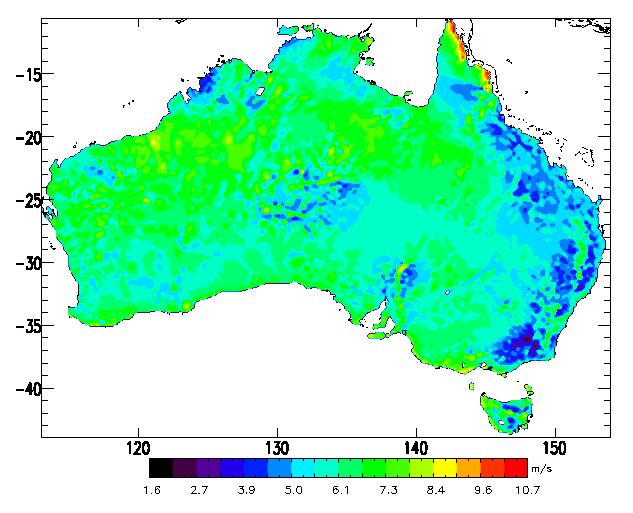
\includegraphics{Figures/winter_u80_average_cont}
\par\end{centering}

\caption{Winter averaged 80m wind speed using the 2010-2011 ACCESS-A meta-level
wind components.\label{fig:Winter-Averaged-U80}}
\end{figure}



\subsection{Optimisation of the Summers in 2010-2011\label{sec:Summer-Only-Optim}}

Figs. \ref{fig:Summer-Only-Installed-Cap} and \ref{fig:Summer-Only-Time-Series}
show the installed capacity and time series output of the optimised
NEM region using only summer data from the ACCESS-A 2010-2011 period.
As suggested earlier, what is clear from Fig. \ref{fig:Summer-Only-Installed-Cap}
is that the characteristics of the installed capacity from the NEM-only
simulation not explained by winter data are explained using the summertime
data. For instance, solar is utilised in the summer-only simulation,
while northern Queensland has no installed capacity of wind power.
Rather, South Australia and north-west Tasmania are preferred locations
for wind power in the summertime. Fig \ref{fig:Summer-Average-U80}
illustrates that the preference for South Australian and north-west
Tasmanian wind is not necessarily as a result of these regions peaking
in the summer (intuitively, this would not make sense and is not seen
in the average plots) but rather as a result of the average wind speeds
dropping off in northern Queensland. 
\begin{figure}[H]
\noindent \begin{centering}
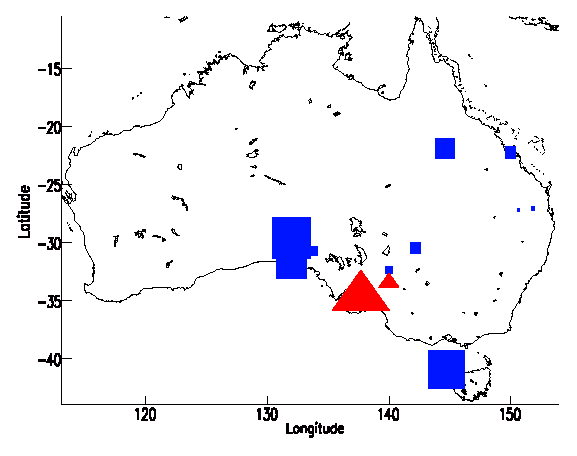
\includegraphics{Figures/asympt_config_full_NEM_east-states_summer-only_11point_wind_21point_dsr_exclusion_raw_demand}
\par\end{centering}

\caption{Installed capacity for the summer-only optimisation of the NEM region.
Blue squares are wind installations that scale according to the largest
installation (11.2GW) and the red triangles are solar installations
that scale according to the largest (8.5GW).\label{fig:Summer-Only-Installed-Cap}}
\end{figure}
\begin{figure}[H]
\noindent \begin{centering}
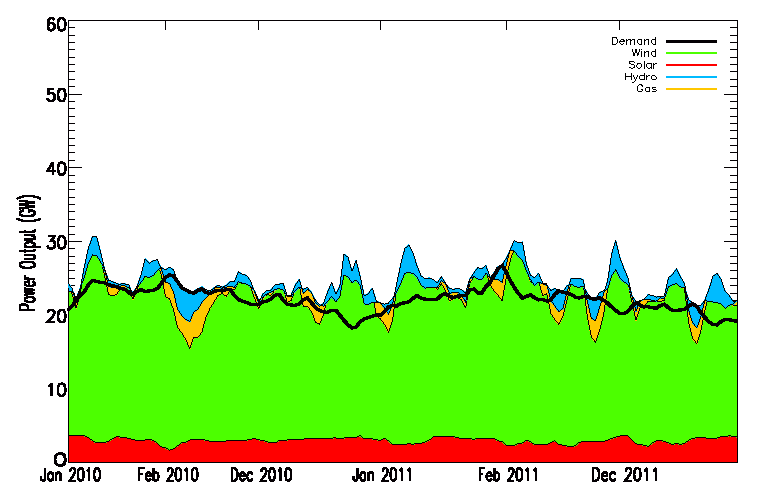
\includegraphics{Figures/GA_output_asympt_config_full_NEM_east-states_summer-only_dist-penlty}
\par\end{centering}

\caption{Daily averaged output from the summer-only simulation of the NEM region.\label{fig:Summer-Only-Time-Series}}
\end{figure}


Table. \ref{tab:Summer-Only-Simulation-Stats} shows that there is
a reduction in the reliance of wind and gas, and an increase (from
zero) in the reliance on solar for the summer-only simulation. Oversupply
is very similar when comparing the summer to the winter-only simulations
(Table. \ref{tab:Oversupp-Comp-Base-Winter-Summer}), but the reduction
in gas usage suggests an overall improved reliability in total RE
during summer.
\begin{table}[H]
\noindent \begin{centering}
\begin{tabular}{|c|c|c|}
\hline 
Resource & Installed Capacity (GW) & Capacity Factor (\%)\tabularnewline
\hline 
\hline 
Wind & 11.4 & 26.3\tabularnewline
\hline 
Solar & 51.5 & 39.3\tabularnewline
\hline 
Hydro & 5 & 33.5\tabularnewline
\hline 
Gas & 14.3 & 7.2\tabularnewline
\hline 
\end{tabular}
\par\end{centering}

\caption{As per Table. \ref{tab:WInter-Only-Simulation-Stats}, except for
the summer-only simulation.\label{tab:Summer-Only-Simulation-Stats}}
\end{table}
\begin{table}[H]
\noindent \begin{centering}
\begin{tabular}{|c|c|c|}
\hline 
Scenario & Maximum Oversupply (GW) & Oversupply Capacity Factor (\%)\tabularnewline
\hline 
\hline 
NEM-Only & 49 & 12.5\tabularnewline
\hline 
Wintertime & 22 & 8\tabularnewline
\hline 
Summertime & 24 & 7.4\tabularnewline
\hline 
\end{tabular}
\par\end{centering}

\caption{Comparison of oversupply statistics between the base NEM-only, winter-only
and summer-only optimisations.\label{tab:Oversupp-Comp-Base-Winter-Summer}}
\end{table}


What is clear from Figs. \ref{fig:Winter-Averaged-U80} and \ref{fig:Summer-Average-U80}
is that the east-coast NEM region has very limited access to average
wind speeds greater than the cut-in wind speed of the GE 2.5MW turbine
of 3ms\textsuperscript{-1}, in both summer and winter. This fact
is unfortunate when considering the major population centres that
the NEM services. What it does suggest though is that a NEM reliant
on a large penetration of wind power needs to consider that it could
be more cost effective to connect remote but high average wind speed
locations to the existing powerline infrastructure. It may not be
sufficient to simply spread-out wind resources across the NEM in the
hope that a diversity in resource can overcome low average output
from a single point. What is more intuitive from Figs. \ref{fig:Winter-Averaged-U80}
and \ref{fig:Summer-Average-U80} (and Fig. \ref{fig:NEM-Only-Installed-Cap})
is that the connection of remote locations to the NEM with high wind
availability, even if the locations are far from population centres,
could be part of the optimal solution for high penetration RE. What
is also clear from the comparison of the seasonal optimisations with
the base NEM-only scenario is that the NEM-only scenario does not
choose to compromise by utilising locations whose output is average
throughout the year. Instead, the NEM-only solution maximised output
by utilising the wintertime maximum in wind for northern Queensland,
and then relying on southern wind installations during summer, irrespective
of the drop-off in wind speed for northern Queensland in Summer. 
\begin{figure}[H]
\noindent \centering{}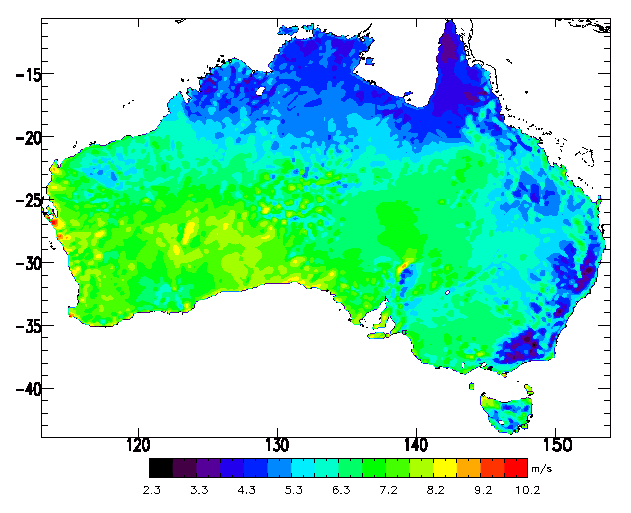
\includegraphics{Figures/summer_u80_average_cont}\caption{Average 80m wind speed for the summer ACCESS-A data of 2010-2011.\label{fig:Summer-Average-U80}}
\end{figure}


Another distinction to make is the southern shift in solar capacity
in the summer-only scenario when compared to the base NEM-only simulation.
In the NEM-only simulation the optimisation chose to install all of
the solar capacity in south-west Queensland. Fig. \ref{fig:All-And-Summer-DSR-Avgs}a
shows that this location has on average some of the best solar availability
in the NEM region. However, the summertime data (Fig. \ref{fig:All-And-Summer-DSR-Avgs}b)
shows a distinct southward shift in the solar maximum (to be expected)
and this is reflected in the choice of location for solar capacity
in the summer-only simulation. In both cases it is sufficient to simply
install capacity at one of the highest average output locations (although
the summer-only scenario uses two adjacent locations, one larger and
one much smaller).
\begin{figure}[H]
\noindent \begin{centering}
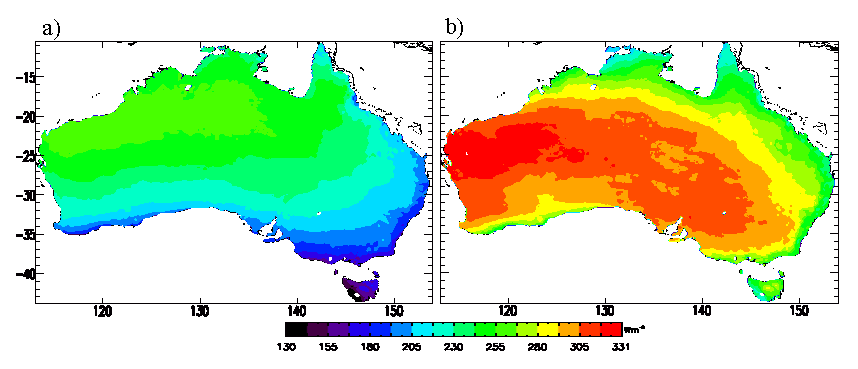
\includegraphics{Figures/all-access_and_summer_dsr_average_cont}
\par\end{centering}

\caption{a) Average DSR for all available ACCESS-A data and b) for the summer
data.\label{fig:All-And-Summer-DSR-Avgs}}
\end{figure}



\section{Optimisation using Larger Transmission Penalties\label{sec:NEM-Only-Extra-Dist-Penalties}}

This section explores the effect on the installed RE capacity (location
and size) of increasing the penalty of connecting to the nearest capital
city. The increased transmission penalties do not take into account
power flow considerations, including voltage and node limitations,
but are used as a guide for the GA to choose locations closer to the
load centres (as per previous simulations). The hypothesis for conducting
simulations with an increased connection cost is to test the quality
of the remote resources. If, for instance, a small increase in penalty
for connecting to the nearest capital city was to drastically contract
RE resources towards the capital cities this would suggest that the
benefit of utilising the higher quality remote resources is minimal.
Contraction of resources towards the capital cities would also suggest
that an alternative near-optimal configuration to that seen in the
NEM-only was possible, but simply not found due to its slight increase
in costs (based on the costs used in the NEM-only simulation). In
this section three increased costs are tested: \$2M/km, \$4M/km and
\$8M/km. In each case the only difference in the configuration of
the electricity model is the increased connection cost for each possible
RE location in the NEM.


\subsection{\$2M/km Connection Cost\label{sub:2X-Optimisation}}

Figs. \ref{fig:2X-Installed-Capacity} and \ref{fig:2X-Time-Series}
depict the installed capacity and time series output using the distance
to nearest capital city cost of \$2M/km (hereafter referred to the
2X simulation). What is clear from Fig. \ref{fig:2X-Installed-Capacity}
is that the increase from \$1M/km to \$2M/km has not significantly
altered the optimal configuration (see Fig. \ref{fig:NEM-Only-Installed-Cap}
for comparison). In the 2X simulation solar PV is still utilised,
as is wind in northern Queensland and a variety of southern wind locations.
\begin{figure}[H]
\noindent \centering{}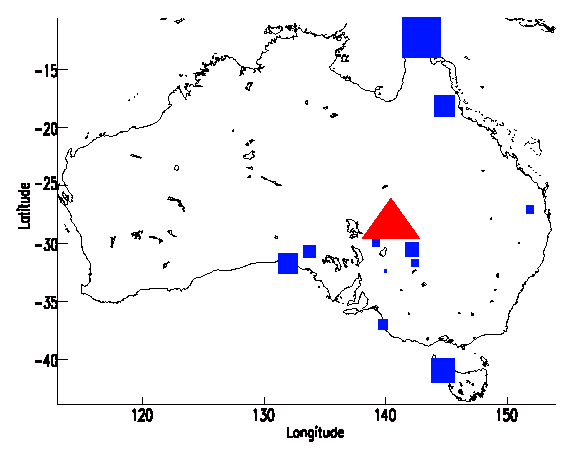
\includegraphics{Figures/asympt_config_full_NEM_east-states_2xdist_11point_wind_21point_dsr_exclusion_raw_demand}\caption{Installed wind (blue squares) and solar (red triangle) capacity and
location. Largest square is 17.3GW and the triangle is 4.2GW.\label{fig:2X-Installed-Capacity} }
\end{figure}
\begin{figure}[H]
\noindent \centering{}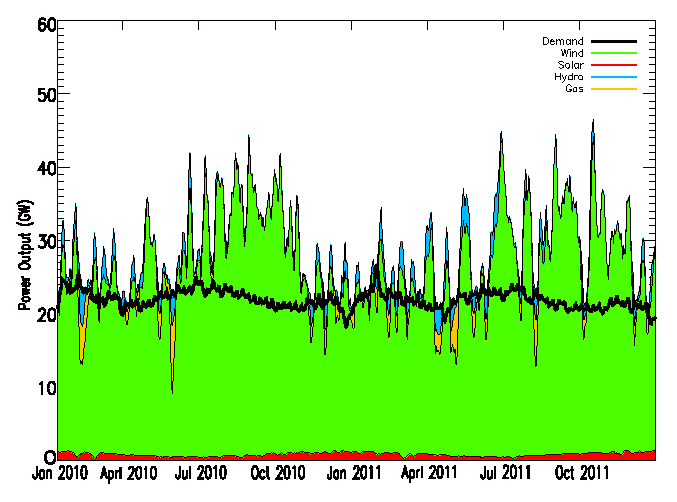
\includegraphics{Figures/GA_output_asympt_config_full_NEM_east-states_2xdist_dist-penlty}\caption{Daily average time series output for the 2X simulation of the NEM
region. \label{fig:2X-Time-Series}}
\end{figure}


Table. \ref{tab:2X-Simulation-Stats} also illustrates a negligible
difference in total installed capacity of each resource, as well as
the capacity factor of those resources in total, when compared to
the original NEM-Only simulation. Thus what is clear from the 2X simulation
is that the high installed capacity at remote locations in the the
NEM-only simulation is a robust solution. Similar locations are utilised
in the 2X simulation in spite of a doubling in the transmission penalty
for connecting such remote locations.
\begin{table}[H]
\noindent \begin{centering}
\begin{tabular}{|c|c|c|}
\hline 
Resource & Capacity (GW) & Capacity Factor (\%)\tabularnewline
\hline 
\hline 
Wind & 71.8 & 37.2\tabularnewline
\hline 
Solar & 4.2 & 20\tabularnewline
\hline 
Hydro & 5 & 24.8\tabularnewline
\hline 
Gas & 17.5 & 5.3\tabularnewline
\hline 
\end{tabular}
\par\end{centering}

\caption{Simulation statistics for the 2X scenario.\label{tab:2X-Simulation-Stats}}
\end{table}
\begin{table}[H]
\noindent \begin{centering}
\begin{tabular}{|c|c|c|}
\hline 
Scenario & Maximum Oversupply (GW) & Oversupply Capacity Factor (\%)\tabularnewline
\hline 
\hline 
NEM-Only & 49 & 12.5\tabularnewline
\hline 
2X & 48 & 12.8\tabularnewline
\hline 
\end{tabular}
\par\end{centering}

\caption{Comparison of oversupply statistics between the base NEM-only and
2X optimisations.\label{tab:Oversupp-Comp-Base-2X}}
\end{table}



\subsection{\$4M/km Connection Cost\label{sub:4X-Optimisation}}

In this section the cost of connecting to the nearest capital city
for each of the locations in the NEM region of the ACCESS-A grid is
further increased to \$4M/km (hereafter referred to as the 4X simulation).
Figs. \ref{fig:4X-Intsalled-Capacity} and \ref{fig:4X-Time-Series}
show the installed capacity and time series output of the optimised
solution to the 4X simulation. Immediately obvious from Fig. \ref{fig:4X-Intsalled-Capacity}
is the loss of any solar capacity. Clearly the advantage of having
solar connected to the NEM is not enough to warrant the extra cost
of connecting the previously installed locations. It is surprising
though that there appears to be no solar resource close enough to
a capital city to warrant some installed capacity. The map of average
DSR (Fig. \ref{fig:All-And-Summer-DSR-Avgs}) demonstrates that on
average the solar resource does not have a large spatial variance
across the Australian continent. In turn the output from nearby locations
would be expected to correlate highly. Therefore the advantage in
having any solar installed in the NEM without storage capacity is
questionable.
\begin{figure}[H]
\noindent \begin{centering}
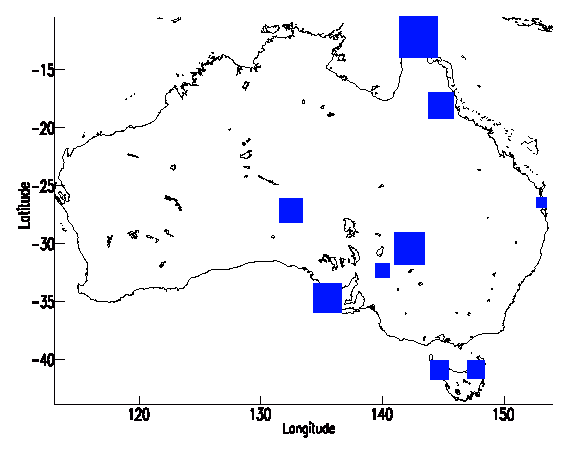
\includegraphics{Figures/asympt_config_full_NEM_east-states_4xdist_11point_wind_21point_dsr_exclusion_raw_demand}
\par\end{centering}

\caption{Installed wind (blue squares) capacity for the optimised NEM region
using the \$4M/km connection cost. Largest square is 14.3GW.\label{fig:4X-Intsalled-Capacity}}
\end{figure}
\begin{figure}[H]
\noindent \begin{centering}
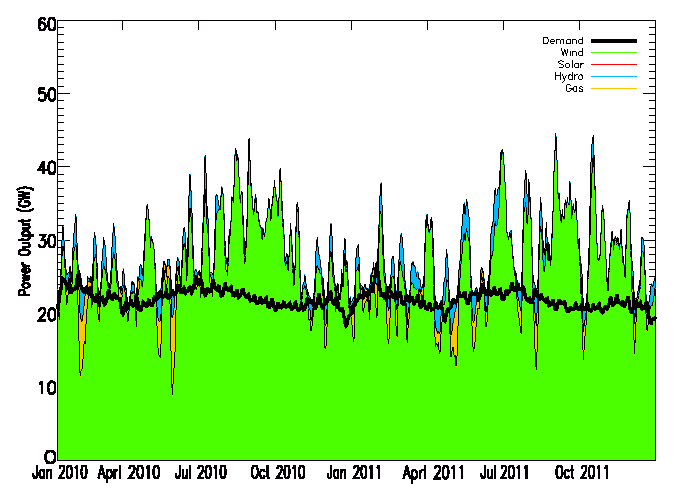
\includegraphics{Figures/GA_output_asympt_config_full_NEM_east-states_4xdist_dist-penlty}
\par\end{centering}

\caption{Daily average time series output of the 4X simulation of the NEM region.\label{fig:4X-Time-Series}}
\end{figure}
 

In terms of the wind installations in the 4X scenario it seems that
similar regions are utilised when compared to both the 2X and NEM-only
simulations. Most of the wind capacity is installed in northern Queensland,
SA and Tasmania in the 4X scenario. There is also a slight increase
in total installed wind capacity (Table. \ref{tab:4X-Simulation-Stats}),
a small increase in gas usage and a small decrease in oversupply in
the 4X scenario when compared to 2X (Table. \ref{tab:Oversupp-Comp-Base-2X-4X}).
Despite little change in the performance of the 4X simulation there
is a noticeable loss of the smaller wind sites utilised in 2X. Increasing
the distance penalty in 4X shows that some of the wind sites utilised
in 2X were limited in their benefit to the system. The increased connection
penalty and the fact that system reliability is maintained in 4X indicates
the contraction of wind resources to larger installations is a cost
effective option (assuming a slight increase in gas usage is acceptable).
This point is further explored in the next section where the connection
cost is increased to \$8M/km.
\begin{table}[H]
\noindent \begin{centering}
\begin{tabular}{|c|c|c|}
\hline 
Resource & Capacity (GW) & Capacity Factor (\%)\tabularnewline
\hline 
\hline 
Wind & 75.3 & 35.8 \tabularnewline
\hline 
Solar & 0 & 0\tabularnewline
\hline 
Hydro & 5 & 26.1\tabularnewline
\hline 
Gas & 20.9 & 5.3\tabularnewline
\hline 
\end{tabular}
\par\end{centering}

\caption{Simulation statistics for the 4X optimisation of the NEM region.\label{tab:4X-Simulation-Stats}}
\end{table}
\begin{table}[H]
\noindent \begin{centering}
\begin{tabular}{|c|c|c|}
\hline 
Scenario & Maximum Oversupply (GW) & Oversupply Capacity Factor (\%)\tabularnewline
\hline 
\hline 
NEM-Only & 49 & 12.5\tabularnewline
\hline 
2X & 48 & 12.8\tabularnewline
\hline 
4X & 46.5 & 12.2\tabularnewline
\hline 
\end{tabular}
\par\end{centering}

\caption{Comparison of oversupply statistics between the base NEM-only, 2X
and 4X optimisations.\label{tab:Oversupp-Comp-Base-2X-4X}}
\end{table}



\subsection{\$8M/km Connection Cost\label{sub:8X-Optimisation}}

Figs. \ref{fig:8X-Installed-Capacity} and \ref{fig:8X-TIme-Series}
show the installed capacity and time series output of the simulation
with the connection cost increased to \$8M/km (hereafter referred
to as the 8X simulation). What is very obvious from Fig. \ref{fig:8X-Installed-Capacity}
is that the connection cost of \$8M/km has crossed a threshold whereby
the optimisation chooses to drastically limit the number of wind sites.
This contraction of resources to four main regions indicates that
any advantage gained by having smaller contributing wind sites in
earlier scenarios is lost if the cost of connecting those sites is
high enough. Table. \ref{tab:8X-Simulation-Stats} illustrates that
while there is very little change in the total wind capacity installed
from 4X to 8X the contraction to four main locations and the subsequent
increase in exposure to wind events (including the capturing of a
cold front passing through South Australia only once, rather than
several times) is covered by an increased use of gas back-up.
\begin{figure}[H]
\noindent \begin{centering}
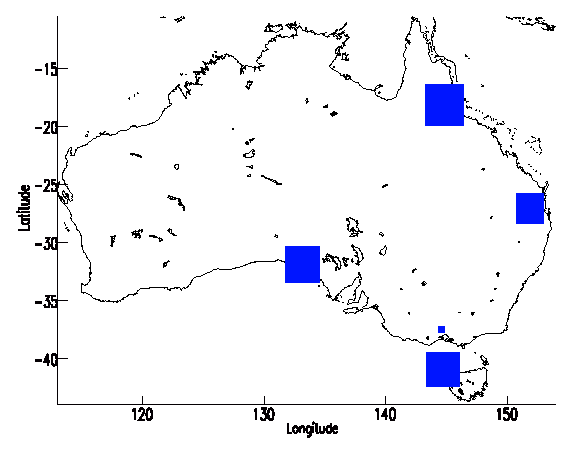
\includegraphics{Figures/asympt_config_full_NEM_east-states_8xdist_11point_wind_21point_dsr_exclusion_raw_demand}
\par\end{centering}

\caption{Installed wind (blue squares) capacity and location for the 8X optimisation
of the NEM region. The largest square represents a 19.9GW installation.\label{fig:8X-Installed-Capacity}}
\end{figure}
\begin{figure}[H]
\noindent \begin{centering}
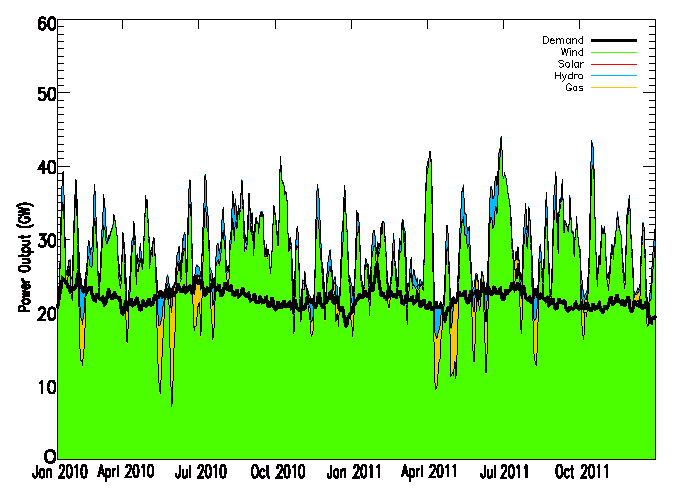
\includegraphics{Figures/GA_output_asympt_config_full_NEM_east-states_8xdist_dist-penlty}
\par\end{centering}

\caption{Daily average time series output of the optimised 8X NEM region simulation.\label{fig:8X-TIme-Series}}
\end{figure}


Comparing values in Table. \ref{tab:Oversupp-Comp-Base-2X-4X-8X}
reveals that the oversupply statistics are relatively unchanged with
respect to connection cost. However, the installed gas capacity increases
from 16.7GW in the NEM-only simulation to 24.7GW in the 8X simulation.
The increased reliance on gas is also visible when comparing the time
series output from the 2X-8X scenarios (Figs. \ref{fig:2X-Time-Series},
\ref{fig:4X-Time-Series} and \ref{fig:8X-TIme-Series}). There is
a clear increase in the number and magnitude of moments when RE dips
below demand as the connection cost increases. Thus it is possible
to conclude that the role of smaller wind installations, and also
the solar installation in 2X, is to cover some of the larger dips
in wind output from the larger wind installations. And that this loss
in diversity of output is covered by an increase in the gas output.
\begin{table}[H]
\noindent \begin{centering}
\begin{tabular}{|c|c|c|}
\hline 
Resource & Capacity (GW) & Capacity Factor (\%)\tabularnewline
\hline 
\hline 
Wind & 72.5 & 37.3\tabularnewline
\hline 
Solar & 0 & 0\tabularnewline
\hline 
Hydro & 5 & 26.8\tabularnewline
\hline 
Gas & 24.7 & 6\tabularnewline
\hline 
\end{tabular}
\par\end{centering}

\caption{Simulation statistics for the 8X scenario.\label{tab:8X-Simulation-Stats}}
\end{table}
\begin{table}[H]
\noindent \begin{centering}
\begin{tabular}{|c|c|c|}
\hline 
Scenario & Maximum Oversupply (GW) & Oversupply Capacity Factor (\%)\tabularnewline
\hline 
\hline 
NEM-Only & 49 & 12.5\tabularnewline
\hline 
2X & 48 & 12.8\tabularnewline
\hline 
4X & 46.5 & 12.2\tabularnewline
\hline 
8X & 46.1 & 13.4\tabularnewline
\hline 
\end{tabular}
\par\end{centering}

\caption{Comparison of oversupply statistics between the base NEM-only, 2X,
4X and 8X optimisations.\label{tab:Oversupp-Comp-Base-2X-4X-8X}}
\end{table}


What is also clear is that despite the increase in reliance on gas
when the connection cost is increased the difference between RE output
and demand for all two-year scenarios presented is minimal (Fig. \ref{fig:RE-Demand-Comparison-All-TransCosts}).
Fig. \ref{fig:RE-Demand-Comparison-All-TransCosts} suggests that
the NEM region as a whole is affected by the same large-scale wind
events and that no amount of strategic resource placement is able
to avoid exposure to such synoptic scale phenomena. What Fig. \ref{fig:RE-Demand-Comparison-All-TransCosts},
in combination with Fig. \ref{fig:8X-Installed-Capacity}, also shows
is that the NEM region can be split into four distinct wind regions---the
four major stations in Fig. \ref{fig:8X-Installed-Capacity}. These
four large stations in the 8X scenario represent most of the RE variance
seen in the earlier 4X, 2X and NEM-only simulations. 
\begin{figure}[H]
\noindent \begin{centering}
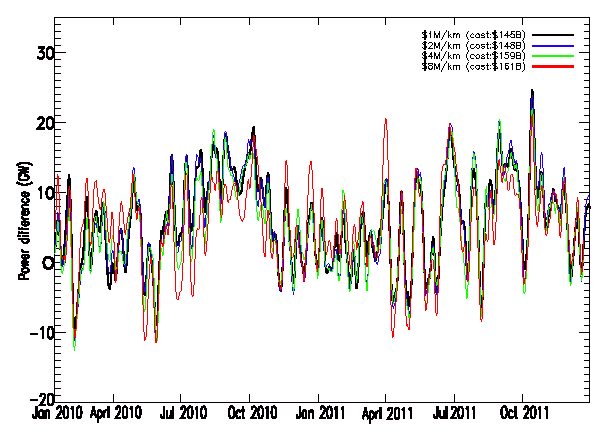
\includegraphics{Figures/RE-demand_comparisons_various_dits-penalties}
\par\end{centering}

\caption{Comparison of daily average RE - demand for the simulations using
four different connection costs. Total cost of the system is indicated
in the legend.\label{fig:RE-Demand-Comparison-All-TransCosts} }
\end{figure}


The four distinct wind regions can also be identified by Fig. \ref{fig:U80-Decorrelation-Major-Locations}.
Fig. \ref{fig:U80-Decorrelation-Major-Locations} illustrates the
decorrelation of each of the four major wind locations in 8X, via
a point correlation map. Each of the four major wind locations from
8X reach correlation values close to zero at distances equal to their
nearest station. Table. \ref{tab:8X-Wind-Power-Correlation} shows
that the largest correlation between any of the four large wind installations
from 8X is 0.07 (between the site near Townsville and the site near
Brisbane).
\begin{figure}[H]
\noindent \begin{centering}
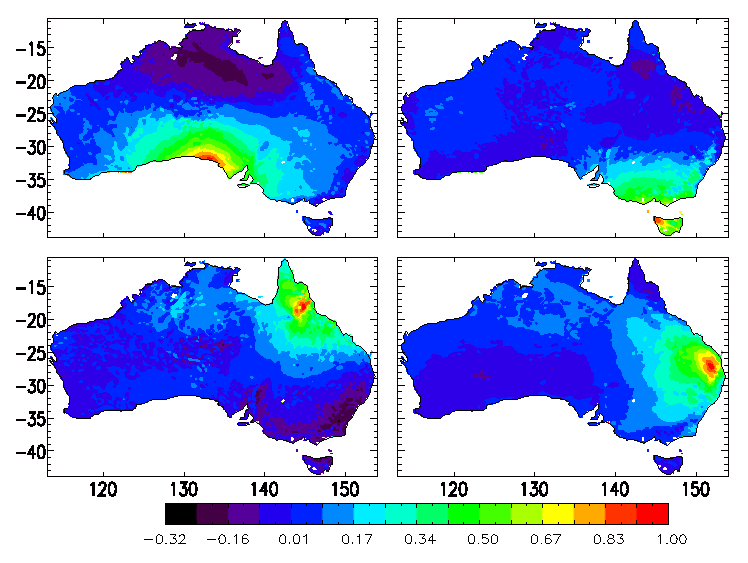
\includegraphics{Figures/ACCESS_u80_decorrel_large_install_regions}
\par\end{centering}

\caption{Point correlation maps using the four major installations from the
8X simulation as anchor points. Regressions are of the 80m wind speed
for the ACCESS-A 2010-2011 data.\label{fig:U80-Decorrelation-Major-Locations}}
\end{figure}


Further comparison between the base NEM-only scenario and the 8X scenario
indicates that three of the four major locations utilised in the 8X
were also utilised, but to a lesser extent, in the NEM-only scenario.
This finding suggests that the optimisation was able to identify the
independent wind regions in the standard transmission cost scenario,
but that it took a large increase in transmission costs before the
model was `willing' to sample those regions at only one location each.
Similar decorrelation characteristics can be found if the installations
utilised in the NEM-only scenario are group together to form one time
series for each 8X region. Table. \ref{tab:NEM-Only-Cluster-Correlations}
shows that each such cluster of smaller stations from the NEM-only
scenario is at most correlated to a value of 0.09. Further evidence
is thus provided for the existence of four distinct wind regions across
the NEM region. 
\begin{table}[H]
\noindent\resizebox{\textwidth}{!}{%

\noindent \begin{centering}
\begin{tabular}{|c|c|c|c|c|}
\hline 
 & Townsville & Brisbane & South Australia & North-west Tasmania\tabularnewline
\hline 
\hline 
Townsville & 1 & 0.071 & 0.038  & -0.058 \tabularnewline
\hline 
Brisbane & 0.071 & 1 & 0.023  & 0.001 \tabularnewline
\hline 
South Australia & 0.038  & 0.023  & 1 & 0.043 \tabularnewline
\hline 
North-west Tasmania & -0.058  & 0.001  & 0.043  & 1\tabularnewline
\hline 
\end{tabular}
\par\end{centering}

}

\caption{Correlation of wind power output from the four major installations
of the 8X simulation.\label{tab:8X-Wind-Power-Correlation}}
\end{table}
\begin{table}[H]
\noindent\resizebox{\textwidth}{!}{%%
\begin{tabular}{|c|c|c|c|c|}
\hline 
 & Townsville cluster & Brisbane & South Australian cluster & North-west Tasmanian cluster\tabularnewline
\hline 
\hline 
Townsville cluster & 1 & 0.077  & -0.025  & 0.061 \tabularnewline
\hline 
Brisbane & 0.077  & 1 & 0.044  & 0.033 \tabularnewline
\hline 
South Australian cluster & -0.025  & 0.044  & 1 & 0.091 \tabularnewline
\hline 
North-west Tasmanian cluster & 0.061  & 0.033  & 0.091  & 1\tabularnewline
\hline 
\end{tabular}

}

\caption{Correlations between clusters from the original NEM-only simulation
with a connection cost of \$1M/km. Each installation from the original
simulation was assigned to a cluster based on which of the four major
locations from the 8X simulation they were nearest to.\label{tab:NEM-Only-Cluster-Correlations}}
\end{table}



\section{Conclusion}

This chapter presents an analysis of the covariance of the wind and
solar fields via the simulation of an highly renewable electricity
dependent electrical network for, initially all of Australia, and
then just eastern Australia (the NEM region). Based on the costs used
the optimisation of the whole of Australia produced a network of wind
and solar stations spread throughout much of western and northern
Australia. No connection cost that was tested was large enough to
discourage the use of such remote locations (not shown) and thus the
choice was made to limit the site selection to the participating states
of the NEM, which services the vast majority of Australia's population.
A base case was created for the NEM, termed the NEM-only scenario.
Analysis of the output from the NEM-only scenario showed that two
weather types (high centred south of WA and a heat low centred in
the north west of WA) were associated with, while two other weather
types (troughs through central and western Australia) were never associated
with, very low RE output. Various alternatives were then tested in
order to gauge the robustness of the NEM-only solution and in order
to reveal any seasonality in the region. Summer-only and winter-only
simulations indicated that the Australian region experiences very
distinct seasonal resource availability, with a very clear maximum
in wind speed in northern Queensland during winter. Solar PV without
storage was shown to be uncompetitive, at current costs, in the winter.
Increasing the cost of transmission to \$2M/km, \$4M/km and \$8M/km
from \$1M/km also resulted in the loss of any installed solar capacity,
along with a contraction of wind resources to four separate regions
with one large installation each. The similarity in solution from
the 2X in comparison to the NEM-only scenario illustrated a robustness
in the NEM-only solution and transmission cost. The larger transmission
costs also demonstrated that the smaller, dispersed, wind installations
seen in the NEM-only base case were not needed if a small increase
in gas usage was possible. However, analysis of the locations used
in the NEM-only scenario showed that the optimiser, even at small
transmission cost, was able to identify and utilise the synoptic scale
wind variance. Correlating the four distinct wind regions showed a
very small amount of shared variance, while maps of the decorrelation
of the wind field demonstrated a decorrelation length scale of approximately
the distance between each region's nearest neighbour (\textasciitilde{}884km).
\end{document}
